\documentclass{llncs}

\usepackage{xcolor}
\usepackage{enumitem,amsmath,amssymb}
\usepackage{url}    % used for \url
\usepackage[linesnumbered,boxed,noline,noend]{algorithm2e}
\def\defaultHypSeparation{\hskip.1in}

\usepackage{tikz}
\usepackage{subfig}
\usepackage{array,booktabs,multirow}
\usepackage{placeins}

\usepackage{logictools}
\usepackage{prooftheory}
\usepackage{comment}
\usepackage{mathenvironments}
\usepackage{drawproof}

\renewcommand{\topfraction}{0.85}
\renewcommand{\textfraction}{0.1}
\renewcommand{\floatpagefraction}{0.75}

\title{Compression of Propositional Resolution Proofs by Lowering Subproofs}

\author{
  Joseph Boudou\inst{1}
  \thanks{Supported by the Google Summer of Code 2012 program.}
  \and 
  Bruno Woltzenlogel Paleo\inst{2}
  \thanks{Supported by the Austrian Science Fund, project P24300.}
}

\authorrunning{J.\~Boudou \and B.\~Woltzenlogel Paleo}

\institute{
  Universit\'e Paul Sabatier, Toulouse \\
  \email{joseph.boudou@matabio.net}
  \and 
  Vienna University of Technology \\
  \email{bruno@logic.at}
}




\begin{document}

\maketitle


\begin{abstract}
This paper describes a generalization of the {\LowerUnits} algorithm \cite{LURPI} for the
compression of propositional resolution proofs.  The generalized algorithm, called
{\LowerUnivalents}, is able to lower not only units but also subproofs of non-unit clauses, provided
that they satisfy some additional conditions.  This new algorithm is particularly suited to be
combined with the {\RecyclePivotsIntersection} algorithm \cite{LURPI}.  A formal proof that
{\LowerUnivalents} always compresses more than {\LowerUnits} is shown, and both algorithms are
empirically compared on thousands of proofs produced by the SMT-Solver \veriT.
\end{abstract}

\setcounter{footnote}{0}

\section{Introduction}

Propositional resolution is among the most successful proof calculi for automated deduction in propositional logic available today. It provides the foundation for DPLL- and CDCL-based Sat/SMT-solvers \cite{veriT}, which perform surprisingly well in practice \cite{sat-competition}, despite the NP-completeness of propositional satisfiability \cite{cook} and the theoretical difficulty associated with NP-complete problems. 

Resolution refutations can also be output by Sat/SMT-solvers with an acceptable efficiency overhead and are detailed enough to allow easy implementation of efficient proof checkers. They can, therefore, be used as certificates of correctness for the answers provided by these tools in case of unsatisfiability.

However, as the refutations found by Sat/SMT-solvers are often redundant, techniques for
compressing and improving resolution proofs in a post-processing stage have flourished.  Algebraic properties of the resolution
operation that might be useful for compression were investigated in \cite{bwp10}.
Compression algorithms based on rearranging and sharing chains of resolution inferences have been
developed in \cite{Amjad07} and \cite{Sinz}.  Cotton \cite{CottonSplit} proposed an algorithm that
compresses a refutation by repeteadly splitting it into a proof of a heuristically chosen literal $\ell$
and a proof of $\dual{\ell}$, and then resolving them to form a new refutation.  The {\ReduceReconstruct} algorithm \cite{RedRec} searches for locally redundant
subproofs that can be rewritten into subproofs of stronger clauses and with fewer resolution steps.
In \cite{RP08} two linear time compression algorithms are introduced. One of them is a partial
regularization algorithm called {\RecyclePivots}.  An enhanced version of this latter
algorithm, called {\RecyclePivotsIntersection} ({\RPI}), is proposed in \cite{LURPI},
along with a new linear time algorithm called {\LowerUnits}.  These two last algorithms are
complementary and better compression can easily be achieved by sequentially composing them (i.e.
executing one after the other).

In this paper, the new algorithm {\LowerUnivalents}, generalizing {\LowerUnits}, is described. Its achieved
goals are to compress more than {\LowerUnits} and to allow fast \emph{non-sequential}  combination
with {\RPI}. While in a sequential combination one algorithm is simply executed after the other, in
a non-sequential combination, both algorithms are executed simultaneously when the proof is
traversed. Therefore, fewer traversals are needed.

The next section introduces the propositional resolution calculus along with the notations,
operations and some theoretical results used in the paper. Section \ref{sec:LU} briefly describes
the {\LowerUnits} algorithm. In Sect. \ref{sec:LUniv} the new algorithm {\LowerUnivalents} is
introduced and it is proved that it always compresses more than {\LowerUnits}. Section
\ref{sec:LUnivRPI} describes the non-sequential combination of {\LowerUnivalents} and {\RPI}.
Lastly, experimental results are discussed in Sect. \ref{sec:exp}.



\section{Propositional Resolution Calculus}

A \emph{literal} is a propositional variable or the negation of a propositional variable. The
\emph{dual} of a literal $\ell$ is denoted $\dual{\ell}$ (i.e. for any propositional variable $p$,
$\dual{p} = \neg p$ and $\dual{\neg p} = p$). The set of all literals is denoted $\mathcal{L}$. A
\emph{clause} is a set of literals. $\bot$ denotes the \emph{empty clause}.


\newcommand{\axiom}[1]{\widehat{#1}}
\newcommand{\n}{v}
\newcommand{\raiz}[1]{\rho(#1)}

\begin{definition}[Proof] 
\label{def:proof}
A directed acyclic graph $\langle V, E, \clause \rangle$, where $V$ is a set of nodes and $E$ is a
set of edges labeled by literals (i.e. $E \subset V \times \mathcal{L} \times V$ and $\n_1
\xrightarrow{\ell} \n_2$ denotes an edge from node $\n_1$ to node $\n_2$ labeled by $\ell$), is a
proof of a clause $\clause$ iff it is inductively constructible according to the following cases:
%
\begin{enumerate}
  \item If $\Gamma$ is a clause, $\axiom{\Gamma}$ denotes some proof $\langle \{ \n \}, \varnothing,
    \Gamma \rangle$, where $\n$ is a new node.
  \item If $\psi_L$ is a proof $\langle V_L, E_L, \clause_L \rangle$ and
    $\psi_R$ is a proof $\langle V_R, E_R, \clause_R \rangle$ and $\ell$ is a literal such that
    $\dual{\ell} \in \clause_L$ and $\ell \in \clause_R$, then
    $\psi_L \odot_\ell \psi_R$ denotes a proof $\langle V, E, \Gamma \rangle$ s.t.
    \begin{align*}
      V &= V_L \cup V_R \cup \{\n \} \\
      E &= E_L \cup E_R \cup
                    \left\{ \n \xrightarrow{\dual{\ell}} \raiz{\psi_L}, \n \xrightarrow{\ell} \raiz{\psi_R} \right\} \\
     \Gamma &= \left( \clause_L \setminus \left\{ \dual{\ell} \right\} \right) \cup \left( \clause_R
                    \setminus \left\{ \ell \right\} \right)
    \end{align*}
    where $\n$ is a new node and $\raiz{\varphi}$ denotes the root node of $\varphi$.
  \qed
\end{enumerate}
\end{definition}


\newcommand{\Vertices}[1]{V_{#1}}
\newcommand{\Edges}[1]{E_{#1}}
\newcommand{\Conclusion}[1]{\clause_{#1}}

\noindent
If $\psi = \varphi_L \odot_{\ell} \varphi_R$, then $\varphi_L$ and $\varphi_R$ are \emph{direct
subproofs} of $\psi$ and $\psi$ is a \emph{child} of both $\varphi_L$ and $\varphi_R$. The
transitive closure of the direct subproof relation is the \emph{subproof} relation. A subproof which
has no direct subproof is an \emph{axiom} of the proof. Contrary to the usual graph and proof
theoretic conventions but following the actual implementation of the data structures used by
\LowerUnivalents, edges are directed from children (resolvents) to their parents (premises).
%
$\Vertices{\psi}$, $\Edges{\psi}$ and $\Conclusion{\psi}$
denote, respectively, the nodes, edges and proved clause (conclusion) of $\psi$.

\newcommand{\Active}[2]{A_{#2}(#1)}
\begin{definition}[Active literals]
Given a proof $\psi$, the set of active literals $\Active{\varphi}{\psi}$ of a subproof $\varphi$
are the labels of edges coming into $\varphi$'s root: 
$$
\Active{\varphi}{\psi} =
  \{\ell \ | \ \exists \varsigma \in \Vertices{\psi}. \ \varsigma \xrightarrow{\ell} \raiz{\varphi} \}
$$
\end{definition}

\SetKwFunction{Rec}{delete}
\SetKw{Let}{let}


Two operations on proofs are used in this paper: the resolution operation~$\odot_\ell$ introduced
above and the deletion of a set of subproofs from a proof, denoted
$\dn{\psi}{\varphi_1 \ldots \varphi_n}$ where $\psi$ is the whole proof and $\varphi_i$ are the
deleted subproofs. Algorithm \ref{algo:del} describes the deletion operation, with
$\dn{\psi}{\varphi_1 \ldots \varphi_n}$ being the result of \Rec{$\psi$,$\{\varphi_1, \ldots ,
\varphi_n\}$}. Both the resolution and deletion operations are considered to be left associative.

\begin{algorithm}[bt]
  \KwIn{a proof $\varphi$}
  \KwIn{$D$ a set of subproofs}
  \KwOut{a proof $\varphi'$ obtained by deleting the subproofs in $D$ from $\varphi$}
  \BlankLine

  \newcommand{\fixL}{\ensuremath{\varphi'_L}}
  \newcommand{\fixR}{\ensuremath{\varphi'_R}}

  \uIf{$\varphi \in D$ or $\raiz{\varphi}$ has no premises}{
    \Return{$\varphi$} \;
  }
  \BlankLine

  \Else{
    \Let{$\varphi_L$, $\varphi_R$ and $\ell$} be such that
      $\varphi = \varphi_L \odot_\ell \varphi_R$ \;
    \Let{$\varphi'_L = $ \Rec{$\varphi_L$,$D$}} \;
    \Let{$\varphi'_R = $ \Rec{$\varphi_R$,$D$}} \;
    \BlankLine

    \uIf{$\varphi'_L \in D$}
      { \Return{\fixR} \; }
    \uElseIf{$\varphi'_R \in D$}
      { \Return{\fixL} \; }
    \BlankLine

    \uElseIf{$\dual{\ell} \notin \Conclusion{\fixL}$}
      { \Return{\fixL} \; }
    \uElseIf{$\ell \notin \Conclusion{\fixR}$}
      { \Return{\fixR} \; }
    \BlankLine

    \Else{ \Return{ \fixL~$\odot_\ell$~\fixR} \; }
  }

  \caption[.]{\FuncSty{delete}}
  \label{algo:del}
\end{algorithm}

The deletion algorithm is a minor variant of the \textsc{Reconstruct-Proof} algorithm presented in
\cite{RP11}.
The basic idea is to traverse the proof in a top-down manner, replacing
each subproof having one of its premises marked for deletion (i.e. in $D$) by its other direct
subproof. The special case when both $\varphi'_L$ and $\varphi'_R$ belong to $D$ is treated rather
implicitly and deserves an explanation: in such a case, one might intuitively expect the result
$\varphi'$ to be undefined and arbitrary. Furthermore, to any child of $\varphi$, $\varphi'$ ought
to be seen as if it were in $D$, as if the deletion of $\varphi'_L$ and $\varphi'_R$ propagated to
$\varphi'$ as well. Instead of assigning some arbitrary proof to $\varphi'$ and adding it to $D$,
the algorithm arbitrarily returns (in line 8) $\varphi'_R$ (which is already in $D$) as the result
$\varphi'$. In this way, the propagation of deletion is done automatically and implicitly. For
instance, the following hold:
\begin{align}
  \dn{\varphi_1 \odot_\ell \varphi_2}{\varphi_1, \varphi_2} &= \varphi_2 \label{eq:exampledel1} \\
\dn{\varphi_1 \odot_\ell \varphi_2 \odot_{\ell'} \varphi_3}{\varphi_1, \varphi_2} &=
  \dn{\varphi_3}{\varphi_1, \varphi_2} \label{eq:exampledel2}
\end{align}
A side-effect of this clever implicit propagation of deletion is that the actual result of deletion
is only meaningful if it is not in $D$. In the example (\ref{eq:exampledel1}), as $\dn{\varphi_1
\odot_\ell \varphi_2}{\varphi_1, \varphi_2} \in \{\varphi_1, \varphi_2\} $, the actual resulting
proof is meaningless. Only the information that it is a deleted subproof is relevant, as it suffices
to obtain meaningful results as shown in (\ref{eq:exampledel2}).

\begin{proposition} \label{prop:del_assoc}
For any proof $\psi$ and any sets $A$ and $B$ of $\psi$'s subproofs,
either $\dn{\psi}{A \cup B}  \in A \cup B$
and    $\dn{\dn{\psi}{A}}{B} \in A \cup B$,
or     $\dn{\psi}{A \cup B} = \dn{\dn{\psi}{A}}{B}$.
\end{proposition}


\begin{definition}[Valent literal]
  In a proof $\psi$, a literal $\ell$ is \emph{valent} for the subproof $\varphi$ iff $\dual{\ell}$
  belongs to the conclusion of $\dn{\psi}{\varphi}$ but not to the conclusion of $\psi$.
\end{definition}

\begin{proposition} \label{prop:valentactive}
In a proof $\psi$, every valent literal of a subproof $\varphi$ is an active literal of $\varphi$.
\end{proposition}

\newcommand{\pedge}[3]{\ensuremath{\raiz{#1} \xrightarrow{#2} \raiz{#3}}}

\begin{proof}
Lines 2, 12, 14 and 16 from Algorithm \ref{algo:del} can not introduce a new literal in the conclusion of
the subproof being processed. Let $\ell$ be a valent literal of $\varphi$ in $\psi$. Because
there is only one subproof to be deleted, $\dual{\ell}$ can only be introduced when processing a
subproof $\varphi'$ such that $\pedge{\varphi'}{\ell}{\varphi}$. \qed
\end{proof}

\begin{proposition}
Given a proof $\psi$ and a set $D = \{\varphi_1 \ldots \varphi_n\}$ of $\psi$'s subproofs, $\forall
\ell \in \mathcal{L}$ s.t. $\ell$ is in the conclusion of $\dn{\psi}{D}$ but not in $\psi$'s
conclusion, then $\exists i$ s.t. $\dual{\ell}$ is a valent literal of $\varphi_i$ in $\psi$.
\end{proposition}


\section{LowerUnits} \label{sec:LU}

When a subproof $\varphi$ has more than one child in a proof $\psi$, it may be possible to \emph{factor} all
the corresponding resolutions: a new proof is
constructed by removing $\varphi$ from $\psi$ and reintroducing it later. The resulting proof is smaller because $\varphi$ participates in a single resolution inference in it (i.e. it has a single child), while in the original proof it participates in as many resolution inferences as the number of children it had. Such a factorization is called \emph{lowering} of $\varphi$, because its delayed reintroduction makes $\varphi$ appear at the bottom of the resulting proof. 

Formally, a subproof $\varphi$ in a proof $\psi$ can be lowered if there exists a proof
$\psi'$ and a literal $\ell$ such that $\psi' = \dn{\psi}{\varphi} \odot_{\ell} \varphi$ and
$\Conclusion{\psi'} \subseteq \Conclusion{\psi}$. It has been noted in \cite{LURPI} that $\varphi$ can always be lowered if it is a \emph{unit}: its conclusion clause has only one literal. This led to the invention of the {\LowerUnits} algorithm, which lowers every unit with more than one child, taking care to reintroduce units in
an order corresponding to the subproof relation: if a unit $\varphi_2$ is a subproof of a unit
$\varphi_1$ then $\varphi_2$ has to be reintroduced later than (i.e. below) $\varphi_1$.

A possible presentation of {\LowerUnits} is shown in Algorithm \ref{algo:LU}. Units are collected
during a first traversal. As this traversal is bottom-up, units are stored in a queue. The traversal
could have been top-down and units stored in a stack. Units are effectively deleted during a second,
top-down traversal. The last for-loop performs the reintroduction of units.

\begin{algorithm}[bt]
  \KwIn {a proof $\psi$}
  \KwOut{a compressed proof $\psi'$}
  \BlankLine

  \SetKwData{Units}{Units}
  \Units $\leftarrow \varnothing$ \;
  \BlankLine

  \For{every subproof $\varphi$ in a bottom-up traversal}{
    \If{$\varphi$ is a unit and has more than one child}{Enqueue $\varphi$ in \Units \; }
  }
  \BlankLine

  $\psi' \leftarrow $ \Rec{$\psi$,$\Units$} \;
  \BlankLine

  \For{every unit $\varphi$ in \Units}{
    \Let{$\{\ell\} = \Conclusion{\varphi}$} \;
    \lIf{$\dual{\ell} \in \Conclusion{\psi'}$}{
    $\psi' \leftarrow \psi' \odot_\ell \varphi$ \;}
  }

  \caption{\LowerUnits}
  \label{algo:LU}
\end{algorithm}




%\FloatBarrier
\section{LowerUnivalents} \label{sec:LUniv}

{\LowerUnits} does not lower every lowerable subproof. In particular, it does not take into
account the already lowered subproofs. For instance, if a unit $\varphi_1$ proving $\{a\}$ has
already been lowered, a subproof $\varphi_2$ with conclusion $\{\neg a, b\}$ may be lowered as well and
reintroduced above $\varphi_1$. The posterior reintroduction of $\varphi_1$ will resolve away $\neg a$ and guarantee that it does not occur in the resulting proof's conclusion. But care must also be taken not to lower $\varphi_2$ if $\neg a$ is a valent literal of
$\varphi_2$, otherwise $a$ will undesirably occur in the resulting proof's conclusion.

\begin{definition}[Univalent subproof]
A subproof $\varphi$ in a proof $\psi$ is \emph{univalent} w.r.t. a set $\Delta$ of literals iff
$\varphi$ has exactly one valent literal $\ell$ in $\psi$, $\ell \notin \Delta$ and
$\Conclusion{\varphi} \subseteq \Delta \cup \left\{ \ell \right\}$. $\ell$ is called the \emph{univalent
literal} of $\varphi$ in $\psi$ w.r.t.  $\Delta$.
\end{definition}

The principle of {\LowerUnivalents} is to lower all univalent subproofs. Having only one valent literal makes them behave essentially like units w.r.t. the technique of lowering. $\Delta$ is
initialized to the empty set. Then the duals of the univalent literals are incrementally added to
$\Delta$. Proposition \ref{prop:LUniv} ensures that the conclusion of the resulting proof
subsumes the conclusion of the original one.

\begin{proposition} \label{prop:LUniv}
Given a proof $\psi$, if 
%for an integer $n$
there is a sequence $U = (\varphi_1 \ldots \varphi_n)$
of $\psi$'s subproofs and a sequence $(\ell_1 \ldots \ell_n)$ of literals such that $\forall i \in
[1 \ldots n]$, $\ell_i$ is the univalent literal of $\varphi_i$ w.r.t. $\Delta_{i-1} =
\{\dual{\ell_1} \ldots \dual{\ell_{i-1}}\}$, then the conclusion of $$ \psi' = \dn{\psi}{U}
\odot_{\ell_n} \varphi_n \ldots \odot_{\ell_1} \varphi_1 $$ subsumes the conclusion of $\psi$.
\end{proposition}

\begin{proof}
The proposition is proven by induction on $n$, along with the fact that $\dn{\psi}{U} \notin U$.
For $n = 0$, $U = \varnothing$ and the properties trivially hold. Suppose a subproof
$\varphi_{n+1}$ of $\psi$ is univalent w.r.t. $\Delta_n$, with univalent literal $\ell_{n+1}$.
Because $\ell_{n+1} \notin \Delta_n$, there exists a subproof of $\dn{\psi}{U}$ with conclusion
containing $\dual{\ell_{n+1}}$, and therefore $\dn{\dn{\psi}{U}}{\varphi_{n+1}} \notin U \cup
\{\varphi_{n+1}\}$.  Let $\Gamma$ be the conclusion of $\dn{\psi}{U}$. The conclusion of $ \psi' =
\dn{\psi}{U \cup \{\varphi_{n+1}\}} = \dn{\dn{\psi}{U}}{\varphi_{n+1}} $ is included in $\Gamma \cup
\{\dual{\ell_{n+1}}\}$. The conclusion of $\psi' \odot_{\ell_{n+1}} \varphi_{n+1}$ is included in
$\Gamma \cup \Delta_n$. As $\Gamma \subseteq \Conclusion{\psi} \cup \Delta_n$, the conclusion of
$\psi' \odot_{\ell_{n+1}} \varphi_{n+1} \ldots \odot_{\ell_1} \varphi_1$ is included in
$\Conclusion{\psi}$. \qed
\end{proof}

For this principle to lead to proof compression, it is important to take care
of the mutual inclusion of univalent subproofs.
%not only of the order in which subproofs are collected for lowering but also of deleting all
%already collected univalent subproofs from the next subproof $\psi_i$ before reintroducing it.
Suppose, for instance, that $\varphi_i, \varphi_j, \varphi_k \in U$, $i < j < k$, $\varphi_j$ is a
subproof of $\varphi_i$ but not a subproof of $\dn{\psi}{\varphi_i}$, and $\dual{\ell_j} \in
\Conclusion{\varphi_k}$.  In this case, $\varphi_j$ will have one more child in
$$
\dn{\psi}{U} \odot_{\ell_n} \varphi_n \ldots \odot_{\ell_k} \varphi_k \ldots \odot_{\ell_j} \varphi_j \ldots \odot_{\ell_i} \varphi_i \ldots \odot_{\ell_1} \varphi_1
$$
than in the original proof $\psi$. The additional child is created when $\varphi_j$ is reintroduced.
All the other children are reintroduced with the reintroduction of $\varphi_i$, because
$\varphi_j$ was not deleted from $\varphi_i$.

To solve this issue, {\LowerUnivalents} traverses the proof in a top-down manner and simultaneously
deletes already collected univalent subproofs, as sketched in Algorithm \ref{algo:LUniv}.  


\SetKwData{Univ}{Univalents}
\begin{algorithm}[bt]
  \KwIn {a proof $\psi$}
  \KwOut{a compressed proof $\psi'$}
  \BlankLine

  \SetKw{Push}{push}
  \SetKw{Pop} {pop}

  \Univ $\leftarrow \varnothing$ \;
  $\Delta \leftarrow \varnothing$ \;
  \BlankLine

  \For{every subproof $\varphi$, in a top-down traversal \label{line:LUniv:step1begin} }{
    $\psi' \leftarrow$ \Rec{$\varphi$,\Univ} \label{line:LUniv:delete} \;
    \If{$\psi'$ is univalent w.r.t. $\Delta$ \label{line:LUniv:lunivtest} }{
      \Let{$\ell$} be the univalent literal \;
      \Push $\dual{\ell}$ onto $\Delta$ \label{line:LUniv:pushDelta} \;
      \Push $\psi'$     onto \Univ \label{line:LUniv:step1end} \;
    }
  }
  \BlankLine

  \tcp{At this point, $\psi' = \dn{\psi}{\Univ}$}
  \While{\Univ $\neq \varnothing$}{ \label{line:LUniv:reintroducebegin}
    $\varphi \leftarrow$ \Pop from \Univ \;
    $\ell \leftarrow$ \Pop from $\Delta$ \;
    \lIf{$\ell \in \Conclusion{\psi'}$ \label{line:LUniv:testreintroduce} }{
    $\psi' \leftarrow \varphi \odot_\ell \psi'$ \;}
  }

  \caption{Simplified \LowerUnivalents}
  \label{algo:LUniv}
\end{algorithm}


Figure \ref{fig:exluniv} shows an example proof and the result of compressing it with \LowerUnivalents. The top-down traversal starts with the leaves (axioms) and only visits a child when all its parents have already been visited. Assuming the unit with conclusion $\{a\}$ is the first visited leaf, it passes the univalent test in line \ref{line:LUniv:lunivtest}, is marked for lowering (line \ref{line:LUniv:step1end}) and the dual of its univalent literal is pushed onto $\Delta$ (line \ref{line:LUniv:pushDelta}). When the subproof with
conclusion $\{\dual{a},b\}$ is considered, $\Delta = \{\dual{a}\}$. As this subproof has only one
valent literal $b \notin \Delta$ and $\{\dual{a},b\} \subseteq \Delta \cup \{b\}$, it is
marked for lowering as well. At this point, $\Delta = \{\dual{a}, \dual{b}\}$, \texttt{Univalents} contains the two subproofs marked for lowering and $\psi'$ is the subproof with conclusion $\{\dual{a}, \dual{b}\}$ shown in Subfig. (b) (i.e. the result of deleting the two marked subproofs from the original proof in Subfig. (a)). No other subproof is univalent; no other subproof is marked for lowering. The final compressed proof (Subfig. (b)) is obtained by reintroducing the two univalent subproofs that had been marked (lines \ref{line:LUniv:reintroducebegin} -- \ref{line:LUniv:testreintroduce}). It has one resolution less than the original. This is so because the subproof with conclusion $\{\dual{a},b\}$ had been used (resolved) twice in the original proof, but lowering delays its use to a point where a single use is sufficient.

\begin{figure}[htb]
  \centering
  \subfloat[Original proof]{
    \centering
    \begin{tikzpicture}

      \rootnode;
      \withchildren{root} {r0}{\dual{a}}  {unit}{a};
      \withchildren{r0}   {r1}{\dual{a},c} {r2}{\dual{a},\dual{c}};
      \withchildren{r1}   {a0}{\dual{b},c} {low}{\dual{a},b};

      \proofnode[above right of=r2] {a1} {\dual{a},\dual{b},\dual{c}};
      \drawchildren {r2} {low} {a1};

    \end{tikzpicture}
  } \qquad
  \centering
  \subfloat[Compressed proof]{
    \centering
    \begin{tikzpicture}

      \rootnode;
      \withchildren{root} {r0}{\dual{a}}          {unit}{a};
      \withchildren{r0}   {r1}{\dual{a},\dual{b}} {low}{\dual{a},b};
      \withchildren{r1}   {a0}{\dual{b},c}        {a1}{\dual{a},\dual{b},\dual{c}};

    \end{tikzpicture}
  }
\caption{Example of proof crompression by \LowerUnivalents} 
\label{fig:exluniv}
\end{figure}


% Discussion of optimizations follow

Although the
call to \FuncSty{delete} inside the first loop (line \ref{line:LUniv:step1begin} to
\ref{line:LUniv:step1end}) suggests quadratic time complexity, this loop (line
\ref{line:LUniv:step1begin} to \ref{line:LUniv:step1end}) can be (and has been) actually implemented
as a recursive function extending a recursive implementation of \FuncSty{delete}. With such an
implementation, {\LowerUnivalents} has a time complexity linear w.r.t. the size of the proof, assuming the
univalent test (at line \ref{line:LUniv:lunivtest}) is performed in constant bounded time. 


Determining whether a literal is valent is expensive. But thanks to Proposition \ref{prop:valentactive},
subproofs with one active literal which is not in $\Conclusion{\psi}$ can be considered instead
of subproofs with one valent literal.  If the active literal is not valent, the corresponding
subproof will simply not be reintroduced later (i.e. the condition in line 28 of Algorithm \ref{algo:fullLUniv} will fail).

While verifying if a subproof could be univalent, some edges might be deleted. If a
subproof $\varphi_i$ has already been collected as univalent subproof with univalent literal
$\ell_i$ and the subproof $\varphi'$ being considered now has $\ell_i$ as active literal, the
corresponding incoming edges can be removed. Even if $\ell_i$ is valent for $\varphi'$, only
$\dual{\ell_i}$ would be introduced, and it would be resolved away when reintroducing
$\varphi_i$. The \FuncSty{delete} operation can be easily modified to remove both nodes and edges.

Algorithm \ref{algo:fullLUniv} sums up the previous remarks for an efficient implementation of
{\LowerUnivalents}. As noticed above, sometimes this algorithm may consider a subproof as univalent when it
is actually not. But as care is taken when reintroducing subproofs (at line \ref{line:full:testreintroduce}),
the resulting conclusion still subsumes the original.  The test that $\ell \in \Conclusion{\varphi}$
at line \ref{line:full:testactive} is mandatory since $\ell$ might have been deleted from
$\Conclusion{\varphi}$ by the deletion of previously collected subproofs.

\begin{algorithm}[pbt]
  \SetAlgoVlined
  \SetAlgoShortEnd

  \KwData {a proof $\psi$, compressed in place}
  \KwIn {a set $D_V$ of subproofs to delete}
  \KwIn {a set $D_E$ of edges to delete}
%  \KwOut{the proof $\psi$ compressed in place}
  \BlankLine

  \SetKw{Push}{push}
  \SetKw{Pop} {pop}
  \SetKw{Add} {add}
  \SetKw{Rep} {replace}

  \SetKwData{Activ}{ActiveLiterals}

  \Univ $\leftarrow \varnothing$ \;
  $\Delta \leftarrow \varnothing$ \;
  \BlankLine

  \For{every subproof $\varphi$, in a top-down traversal of $\psi$ }{

    \tcp{The deletion part.}
    \If{$\varphi$ is not an axiom}{
      \Let{$\varphi = \varphi_L \odot_\ell \varphi_R$} \;
      \uIf{ $\varphi_L \in D_V$ or $\pedge{\varphi}{\dual{\ell}}{\varphi_L} \in D_E$ }{
        \uIf{ $\pedge{\varphi}{\ell}{\varphi_R} \in D_E$ }{
          \Add $\varphi$ to $D_V$ \;
        }
        \Else{
          \Rep $\varphi$ by $\varphi_R$ \;
        }
      }
      \ElseIf{ $\varphi_R \in D_V$ or $\pedge{\varphi}{\dual{\ell}}{\varphi_R} \in D_E$ }{
        \uIf{ $\pedge{\varphi}{\ell}{\varphi_L} \in D_E$ }{
          \Add $\varphi$ to $D_V$ \;
        }
        \Else{
          \Rep $\varphi$ by $\varphi_L$ \;
        }
      }
    }
    \BlankLine
    
    \tcp{Test whether $\varphi$ is univalent.}
    \Activ $\leftarrow \varnothing$ \;
    \For{each incoming edge $e = \n \xrightarrow{\ell} \raiz{\varphi}$, $e \notin D_E$ }{
      \uIf{$\dual{\ell} \in \Delta$}{
        \Add $e$ to $D_E$ \;
      }
      \ElseIf{$\ell \notin \Delta$, $\ell \in \Conclusion{\varphi}$ \label{line:full:testactive}
              and $\ell \notin \Conclusion{\psi}$ }{
        \Add $\ell$ to \Activ \;
      }
    }

%    \BlankLine
    \If{\Activ $= \{\ell\}$ and $\Conclusion{\varphi} \subseteq \Delta \cup \{\ell\}$ }{
      \Push $\dual{\ell}$ onto $\Delta$ \;
      \Push $\varphi$     onto \Univ  \;
    }
  }
  \BlankLine

  \tcp{Reintroduce lowered subproofs.}
  \While{\Univ $\neq \varnothing$}{
    $\varphi \leftarrow$ \Pop from \Univ \;
    $\ell \leftarrow$ \Pop from $\Delta$ \;
    \If{$\ell \in \Conclusion{\psi}$ \label{line:full:testreintroduce}  }{
      \Rep $\psi$ by $\varphi \odot_\ell \psi$ \;}
  }

  \caption{Optimized {\LowerUnivalents} as an enhanced \texttt{delete}}
  \label{algo:fullLUniv}
\end{algorithm}


Every node in a proof $\langle V, E, \Gamma \rangle$ has exactly two outgoing edges unless it is the
root of an axiom. Hence the number of axioms is $|V| - \frac{1}{2}\,|E|$ and because there is at
least one axiom, the average number of active literals per node is strictly less than two.
Therefore, if {\LowerUnivalents} is implemented as an improved recursive \FuncSty{delete}, its time
complexity remains linear, assuming membership of literals to the set $\Delta$ is computed in constant
time.

\begin{proposition} \label{prop:compression}
Given a proof $\psi$,
{\LowerUnits\unskip\FuncSty{(}$\psi$\FuncSty{)}}
has at least as many nodes as 
{\LowerUnivalents\unskip\FuncSty{(}$\psi$\FuncSty{)}}
if there are no two units in $\psi$ with the same conclusion.
\end{proposition}

\begin{proof}
A unit $\varphi$ has exactly one active literal $\ell$. Therefore $\varphi$ is collected by
{\LowerUnivalents} unless $\dual{\ell} \in \Delta$ or $\ell \in \Delta$. If $\dual{\ell} \in \Delta$
all the incoming edges to $\raiz{\varphi}$ are deleted. If $\ell \in \Delta$, every edge
$\n \xrightarrow{\dual{\ell}} \n'$ where $\n$ is on a path from $\raiz{\psi}$ to $\raiz{\varphi}$
is deleted.
%coming from a descendent of $\raiz{\varphi}$ and labeled by $\dual{\ell} are deleted.
In particular, for every edge $\n \xrightarrow{\ell} \raiz{\varphi}$ the edge $\n
\xrightarrow{\dual{\ell}} \n'$ is deleted.  Moreover, as $\ell$ is the only literal of $\varphi$'s
conclusion, $\varphi$ is propagated down the proof until the univalent subproof with valent literal
$\dual{\ell}$ is reintroduced. \qed
\end{proof}

In the case where there are at least two units with the same conclusion in $\psi$, the
compressed proof depends on the order in which the units are collected. For both algorithms, only one of these units appears in the compressed proof.



\section{Remarks about Combining {\LowerUnivalents} with {\RPI}} \label{sec:LUnivRPI}

\begin{definition}[Regular proof \cite{Tseitin}]
A proof $\psi$ is \emph{regular} iff on every path from its root to any of its axioms, each literal
labels at most one edge. Otherwise, $\psi$ is \emph{irregular}.
\end{definition}

Any irregular proof can be converted into a regular proof having the same axioms and the same
conclusion. But it has been proved \cite{Goerdt} that such a total regularization might result in a
proof exponentially bigger than the original. 

Nevertheless, \emph{partial} regularization algorithms, such as {\RecyclePivots} \cite{RP08} and {\RecyclePivotsIntersection} ({\RPI}) \cite{LURPI}, carefully avoid the worst case of total regularization and do efficiently compress proofs.  For
any subproof $\varphi$ of a proof $\psi$, {\RPI} removes the edge $\raiz{\varphi} \xrightarrow{\ell}
\n$ if $\ell$ is a safe literal for $\varphi$.

\begin{definition}[Safe literal]
A literal $\ell$ is \emph{safe} for a subproof $\varphi$ in a proof $\psi$ iff $\ell$ labels at
least one edge on every path from $\raiz{\psi}$ to $\raiz{\varphi}$.
\end{definition}

{\RPI} performs two traversals. During the first one, safe literals are collected and edges are
marked for deletion. The second traversal is the effective deletion similar to the
$\FuncSty{delete}$ algorithm.

Both sequential compositions of {\LowerUnits} with {\RPI} have been shown to achieve good
compression ratio \cite{LURPI}. However, the best combination order ({\LowerUnits} after
{\RPI} (\texttt{LU.RPI}) or {\RPI} after {\LowerUnits} (\texttt{RPI.LU})) depends on the input proof. A reasonable solution is to perform both combinations and then to choose the smallest
compressed proof, but sequential composition is time consuming. To speed up DAG traversal, it is useful to topologically sort the nodes of the graph first. But in case of sequential composition this costly operation has to be done twice. Moreover, some traversals, like deletion, are identical in both algorithms and might be shared. Whereas implementing a non-sequential combination of {\RPI} after {\LowerUnits} is not difficult, a non-sequential combination of {\LowerUnits} after {\RPI} would be complicated. 
The difficulty is that {\RPI} could create some new units which would be visible only after the deletion
phase.  A solution could be to test for units during deletion. But if units are
effectively lowered during this deletion, their deletion would cause some units to become non-units.
And postponing deletions of units until a second deletion traversal would prevent the sharing of
this traversal and would cause one more topological sorting to be performed, because the deletion phase significantly transforms the structure of the DAG.

Apart from having an improved compression ratio, another advantage of {\LowerUnivalents} over
{\LowerUnits} is that {\LowerUnivalents} can be implemented as an enhanced \FuncSty{delete}
operation. With such an implementation, a simple non-sequential combination of {\LowerUnivalents}
after {\RPI} can be implemented just by replacing the second traversal of {\RPI} by
{\LowerUnivalents}. After the first traversal of {\RPI}, as all edges labeled by a safe literal have been marked for deletion, the remaining active literals are all valent, because for every edge $\pedge{\varphi}{\ell}{\varphi'}$, $\ell$ is either a safe literal
of $\varphi$ or a valent literal of $\varphi'$.  Therefore, in the second traversal of the non-sequential combination (deletion enhanced by {\LowerUnivalents}), all univalent subproofs are lowered.



\section{Experiments} \label{sec:exp}

{\LowerUnivalents} and {\LUnivRPI} have been implemented in the functional programming
language Scala\footnote{\url{http://www.scala-lang.org/}} as part of the \skeptik
library\footnote{\url{https://github.com/Paradoxika/Skeptik}}. {\LowerUnivalents} has been implemented as a
recursive \FuncSty{delete} improvement.

The algorithms have been applied to 5\,059 proofs produced by the SMT-solver
{\veriT}\footnote{\url{http://www.verit-solver.org/}} on unsatisfiable benchmarks from the
SMT-Lib\footnote{\url{http://www.smtlib.org/}}.  The details on the number of proofs per SMT category
are shown in Table \ref{tab:benchmarks}.  The proofs were translated into pure resolution proofs by
considering every non-resolution inference as an axiom.

\begin{table}[tb]
  \caption{Number of proofs per benchmark category}
  \label{tab:benchmarks}
  \centering
  \begin{tabular}{lr}
    \toprule
    Benchmark~ &  Number \\
    Category       & ~of Proofs \\
    \midrule
    QF\_UF      & 3907 \\
    QF\_IDL     &  475 \\
    QF\_LIA     &  385 \\
    QF\_UFIDL   &  156 \\
    QF\_UFLIA   &  106 \\
    QF\_RDL     &   30 \\
    \bottomrule
  \end{tabular}
\end{table}

The experiment compared the following algorithms:
\begin{description}
  \item[LU:] the {\LowerUnits} algorithm from \cite{LURPI};
  \item[LUniv:] the {\LowerUnivalents} algorithm;
  \item[RPILU:] a non-sequential combination of {\RPI} after {\LowerUnits};
  \item[RPILUniv:] a non-sequential combination of {\RPI} after {\LowerUnivalents};
  \item[LU.RPI:] the sequential composition of {\LowerUnits} after {\RPI};
  \item[LUnivRPI:] the non-sequential combination of {\LowerUnivalents} after {\RPI} as described in Sect. \ref{sec:LUnivRPI};
  \item[RPI:] the {\RecyclePivotsIntersection} from \cite{LURPI};
  \item[Split:] Cotton's \texttt{Split} algorithm (\cite{CottonSplit});
  \item[RedRec:] the {\ReduceReconstruct} algorithm from \cite{RedRec};
  \item[Best RPILU/LU.RPI:] which performs both \texttt{RPILU} and \texttt{LU.RPI} and chooses the smallest resulting compressed proof;
  \item[Best RPILU/LUnivRPI:] which performs \texttt{RPILU} and \texttt{LUnivRPI} and chooses the smallest resulting
    compressed proof.
\end{description}

For each of these algorithms, the time needed to compress the proof along with the number of nodes
and the number of axioms (i.e. \emph{unsat core} size) have been measured. Raw data of the experiment can be downloaded from {\skeptik}'s repository\footnote{\url{https://raw.github.com/Paradoxika/Skeptik/master/doc/papers/LUniv/all-final.csv}}.

The experiments were executed on the Vienna Scientific Cluster\footnote{\url{http://vsc.ac.at/}}
VSC\nobreakdash-2. Each algorithm was executed in a single core and had up to 16 GB of memory available. This amount of memory has been useful to compress the biggest proofs (with more than $10^6$ nodes).


The overall results of the experiments are shown in Table \ref{tab:average}. The compression ratios
in the second column are computed according to formula (\ref{eq:compression}), in which $\psi$
ranges over all the proofs in the benchmark and $\psi'$ ranges over the corresponding compressed
proofs.
\begin{equation} \label{eq:compression}
  1 - \frac{ \sum {|\Vertices{\psi'}|} }{ \sum {|\Vertices{\psi}|} }
\end{equation}
The unsat core compression ratios are computed in the same way, but using the number of axioms instead of
the number of nodes. The speeds on the fourth column are computed according to formula
(\ref{eq:speed}) in which $d_{\psi}$ is the duration in milliseconds of $\psi$'s compression by a
given algorithm.
\begin{equation} \label{eq:speed}
  \frac{ \sum {|\Vertices{\psi}|} }{ \sum {d_{\psi}} }
\end{equation}

For the \texttt{Split} and \texttt{RedRec} algorithms, which must be repeated, a timeout has
been fixed so that the speed is about 3 nodes per millisecond. 


\begin{table}[tb]
  \caption{Total compression ratios}
  \label{tab:average}
  \centering
  \begin{tabular}{lrrr}
    \toprule
    \multirow{2}{*}{Algorithm} & \multirow{2}{*}{Compression} & Unsat Core    & \phantom{.........}\multirow{2}{*}{Speed} \\
                                             &                                               & \phantom{...}Compression &        \\
    \midrule
    LU                &  7.5 \% &  0.0 \% & 22.4 n/ms \\
    LUniv             &  8.0 \% &  0.8 \% & 20.4 n/ms \\
    RPILU             & 22.0 \% &  3.6 \% &  7.4 n/ms \\
    RPILUniv          & 22.1 \% &  3.6 \% &  6.5 n/ms \\
    LU.RPI            & 21.7 \% &  3.1 \% & 15.1 n/ms \\
    LUnivRPI          & 22.0 \% &  3.6 \% & 17.8 n/ms \\
    RPI               & 17.8 \% &  3.1 \% & 31.3 n/ms \\
    Split             & 21.0 \% &  0.8 \% &  2.9 n/ms \\
    RedRec            & 26.4 \% &  0.4 \% &  2.9 n/ms \\
    Best RPILU/LU.RPI       & 22.0 \% &  3.7 \% &  5.0 n/ms \\
    Best RPILU/LUnivRPI & 22.2 \% &  3.7 \% &  5.2 n/ms \\
    \bottomrule
  \end{tabular}
\end{table}

\newcommand{\va}[1]{\ensuremath{v_{\text{#1}}}}

Figure \ref{fig:LU} shows the comparison of {\LowerUnits} with {\LowerUnivalents}. Subfigures (a) and (b) are scatter plots where each dot represents a single benchmark proof. 
Subfigure (c) is a histogram showing, in the vertical axis, the proportion of proofs having \emph{(normalized) compression ratio difference} within the intervals showed in the horizontal axis. This difference is computed using formula (\ref{eq:histogram}) with \va{LU}
and \va{LUniv} being the compression ratios obtained respectively by {\LowerUnits} and
{\LowerUnivalents}.
\begin{equation} \label{eq:histogram}
  \frac { \va{LU} - \va{LUniv} }{ \frac{\va{LU} + \va{LUniv}}{2} }
\end{equation}
The number of proofs for which $\va{LU} = \va{LUniv}$ is not displayed in the histogram.
The \emph{(normalized) duration differences} in subfigure (d) are computed using the same formula~(\ref{eq:histogram}) but
with \va{LU} and \va{LUniv} being the time taken to compress the proof by {\LowerUnits} and
{\LowerUnivalents} respectively.

\begin{figure}[tb]
  \centering
  \subfloat[Compression ratio]{
    \centering
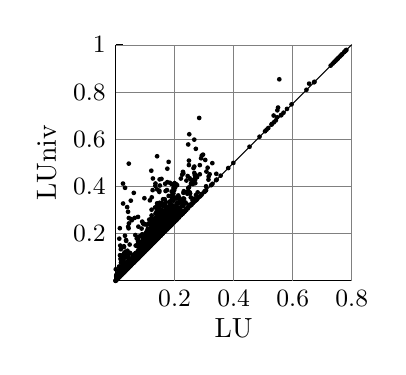
\begin{tikzpicture}

\draw (0,0) -- (3,0);
\node at (1.5,-0.6) {LU};
\node [anchor=north] at (0.75,0) {\small 0.2};
\draw (0.75,0) -- (0.75,0.1);
\draw [style=help lines] (0.75,0) -- (0.75,3);
\node [anchor=north] at (1.5,0) {\small 0.4};
\draw (1.5,0) -- (1.5,0.1);
\draw [style=help lines] (1.5,0) -- (1.5,3);
\node [anchor=north] at (2.25,0) {\small 0.6};
\draw (2.25,0) -- (2.25,0.1);
\draw [style=help lines] (2.25,0) -- (2.25,3);
\node [anchor=north] at (3,0) {\small 0.8};
\draw (3,0) -- (3,0.1);
\draw [style=help lines] (3,0) -- (3,3);
\draw (0,0) -- (0,3);
\node [rotate=90] at (-2.5em,1.5) {LUniv};
\node [anchor=east] at (0,0.599) {\small 0.2};
\draw (0,0.599) -- (0.1,0.599);
\draw [style=help lines] (0,0.599) -- (3,0.599);
\node [anchor=east] at (0,1.198) {\small 0.4};
\draw (0,1.198) -- (0.1,1.198);
\draw [style=help lines] (0,1.198) -- (3,1.198);
\node [anchor=east] at (0,1.797) {\small 0.6};
\draw (0,1.797) -- (0.1,1.797);
\draw [style=help lines] (0,1.797) -- (3,1.797);
\node [anchor=east] at (0,2.396) {\small 0.8};
\draw (0,2.396) -- (0.1,2.396);
\draw [style=help lines] (0,2.396) -- (3,2.396);
\node [anchor=east] at (0,2.995) {\small 1};
\draw (0,2.995) -- (0.1,2.995);
\draw [style=help lines] (0,2.995) -- (3,2.995);
\foreach \pos in {
	(0.000000, 0.000000),
	(0.005240, 0.005240),
	(0.010682, 0.010682),
	(0.015175, 0.015175),
	(0.019519, 0.019519),
	(0.011300, 0.029959),
	(0.019595, 0.028273),
	(0.024510, 0.024510),
	(0.011766, 0.037645),
	(0.028846, 0.028846),
	(0.019449, 0.038898),
	(0.030308, 0.035019),
	(0.036408, 0.036408),
	(0.034538, 0.043075),
	(0.041208, 0.041818),
	(0.008286, 0.060941),
	(0.043578, 0.047670),
	(0.039111, 0.053466),
	(0.049368, 0.050282),
	(0.022477, 0.068865),
	(0.016859, 0.071395),
	(0.010680, 0.074302),
	(0.054051, 0.054154),
	(0.046683, 0.066164),
	(0.058384, 0.058384),
	(0.039416, 0.078186),
	(0.060736, 0.064244),
	(0.055657, 0.072373),
	(0.046408, 0.081664),
	(0.065991, 0.067421),
	(0.052330, 0.079270),
	(0.059494, 0.078548),
	(0.065122, 0.073995),
	(0.027266, 0.096107),
	(0.070894, 0.071107),
	(0.066471, 0.080369),
	(0.057514, 0.087709),
	(0.074950, 0.075947),
	(0.049802, 0.095644),
	(0.041119, 0.099884),
	(0.065398, 0.086684),
	(0.073090, 0.082441),
	(0.079679, 0.079679),
	(0.065648, 0.093650),
	(0.073850, 0.088421),
	(0.054793, 0.102018),
	(0.043824, 0.107619),
	(0.060764, 0.100052),
	(0.080854, 0.086707),
	(0.067071, 0.102366),
	(0.086862, 0.086862),
	(0.081852, 0.094573),
	(0.050777, 0.114381),
	(0.074022, 0.103266),
	(0.089614, 0.092495),
	(0.068716, 0.109486),
	(0.081107, 0.100758),
	(0.061254, 0.115503),
	(0.087183, 0.098250),
	(0.054288, 0.119939),
	(0.038040, 0.126958),
	(0.095093, 0.095395),
	(0.083427, 0.108037),
	(0.093542, 0.101529),
	(0.079141, 0.113669),
	(0.072835, 0.118268),
	(0.045721, 0.131296),
	(0.099775, 0.099775),
	(0.070397, 0.124436),
	(0.090729, 0.111715),
	(0.097880, 0.106648),
	(0.087114, 0.116676),
	(0.002809, 0.146067),
	(0.079539, 0.123544),
	(0.104222, 0.104355),
	(0.095442, 0.116615),
	(0.102629, 0.110546),
	(0.072835, 0.132341),
	(0.108540, 0.108736),
	(0.092309, 0.123067),
	(0.086578, 0.128831),
	(0.104623, 0.116931),
	(0.112820, 0.113157),
	(0.093507, 0.132838),
	(0.111032, 0.119016),
	(0.104301, 0.127636),
	(0.117714, 0.118072),
	(0.093454, 0.139409),
	(0.110423, 0.126945),
	(0.103057, 0.135142),
	(0.116910, 0.124068),
	(0.123373, 0.123847),
	(0.111276, 0.135312),
	(0.117323, 0.130197),
	(0.124177, 0.129868),
	(0.119859, 0.137071),
	(0.068662, 0.169014),
	(0.089438, 0.160375),
	(0.116412, 0.142188),
	(0.095884, 0.156794),
	(0.130244, 0.130693),
	(0.045088, 0.180847),
	(0.126865, 0.137582),
	(0.061123, 0.179488),
	(0.134693, 0.134991),
	(0.111188, 0.156832),
	(0.121036, 0.149412),
	(0.131782, 0.141849),
	(0.096415, 0.168813),
	(0.117763, 0.155382),
	(0.138339, 0.140055),
	(0.080887, 0.181983),
	(0.133837, 0.148182),
	(0.140760, 0.146263),
	(0.129770, 0.156387),
	(0.101752, 0.178496),
	(0.140568, 0.152539),
	(0.124092, 0.166266),
	(0.146779, 0.147280),
	(0.147007, 0.153321),
	(0.112796, 0.180528),
	(0.144330, 0.160438),
	(0.108010, 0.187785),
	(0.130775, 0.173552),
	(0.153846, 0.153846),
	(0.138526, 0.170375),
	(0.151331, 0.160330),
	(0.116438, 0.189604),
	(0.148301, 0.166050),
	(0.159091, 0.159091),
	(0.153552, 0.169284),
	(0.159054, 0.166395),
	(0.132564, 0.189486),
	(0.150860, 0.176181),
	(0.094182, 0.213071),
	(0.166667, 0.166667),
	(0.161309, 0.174369),
	(0.146494, 0.188143),
	(0.068702, 0.230854),
	(0.168686, 0.172947),
	(0.124738, 0.207538),
	(0.160190, 0.182191),
	(0.077376, 0.230050),
	(0.116300, 0.214097),
	(0.166922, 0.179007),
	(0.131261, 0.208117),
	(0.173606, 0.177528),
	(0.159574, 0.194503),
	(0.174016, 0.184222),
	(0.179564, 0.180054),
	(0.165931, 0.193022),
	(0.171103, 0.189532),
	(0.120347, 0.225424),
	(0.161601, 0.200677),
	(0.076732, 0.246686),
	(0.179341, 0.188595),
	(0.185308, 0.185560),
	(0.176153, 0.194376),
	(0.132669, 0.231269),
	(0.182430, 0.195460),
	(0.190081, 0.190793),
	(0.084904, 0.257799),
	(0.072782, 0.261562),
	(0.175120, 0.207888),
	(0.189810, 0.198119),
	(0.194946, 0.194946),
	(0.185239, 0.208139),
	(0.171769, 0.219867),
	(0.191410, 0.206772),
	(0.197353, 0.201440),
	(0.094054, 0.265946),
	(0.147789, 0.241013),
	(0.062797, 0.278281),
	(0.161275, 0.235616),
	(0.184083, 0.219008),
	(0.154805, 0.241902),
	(0.202897, 0.203884),
	(0.192831, 0.218390),
	(0.205231, 0.212015),
	(0.103448, 0.280788),
	(0.192849, 0.230473),
	(0.206108, 0.219084),
	(0.212089, 0.214481),
	(0.185789, 0.241775),
	(0.204179, 0.229419),
	(0.172061, 0.255348),
	(0.215604, 0.222021),
	(0.210520, 0.228547),
	(0.222696, 0.224346),
	(0.212628, 0.234581),
	(0.219582, 0.230989),
	(0.193078, 0.254962),
	(0.228261, 0.228261),
	(0.216663, 0.239534),
	(0.168837, 0.276957),
	(0.133041, 0.296518),
	(0.056493, 0.323925),
	(0.233010, 0.233010),
	(0.194622, 0.268564),
	(0.203616, 0.264023),
	(0.228530, 0.245017),
	(0.236479, 0.238095),
	(0.087494, 0.324280),
	(0.212490, 0.262318),
	(0.204021, 0.270597),
	(0.210021, 0.268504),
	(0.236555, 0.245576),
	(0.231781, 0.250802),
	(0.242110, 0.242110),
	(0.134328, 0.318408),
	(0.230820, 0.257512),
	(0.209390, 0.275701),
	(0.241534, 0.249383),
	(0.247934, 0.247934),
	(0.223259, 0.272292),
	(0.237430, 0.260768),
	(0.160243, 0.314568),
	(0.218291, 0.277480),
	(0.229548, 0.270470),
	(0.243730, 0.258209),
	(0.234504, 0.266870),
	(0.250974, 0.253243),
	(0.249047, 0.261067),
	(0.242545, 0.269783),
	(0.254983, 0.258756),
	(0.218161, 0.292502),
	(0.240307, 0.276518),
	(0.252135, 0.266873),
	(0.260870, 0.260870),
	(0.220285, 0.298421),
	(0.111483, 0.356001),
	(0.260602, 0.268810),
	(0.250028, 0.282343),
	(0.239909, 0.291172),
	(0.258720, 0.275401),
	(0.215543, 0.313621),
	(0.269565, 0.269565),
	(0.272120, 0.275648),
	(0.136600, 0.362996),
	(0.265161, 0.284910),
	(0.243765, 0.303831),
	(0.270900, 0.281833),
	(0.126701, 0.369859),
	(0.260209, 0.293482),
	(0.277923, 0.278696),
	(0.234560, 0.316205),
	(0.222632, 0.326556),
	(0.270852, 0.289003),
	(0.277199, 0.286041),
	(0.252807, 0.307887),
	(0.185896, 0.352863),
	(0.282536, 0.282536),
	(0.268998, 0.301397),
	(0.282000, 0.289685),
	(0.246580, 0.321812),
	(0.066667, 0.400000),
	(0.288462, 0.288462),
	(0.151345, 0.381215),
	(0.278192, 0.301585),
	(0.283743, 0.296460),
	(0.239348, 0.336139),
	(0.291415, 0.294021),
	(0.287822, 0.302328),
	(0.280098, 0.310157),
	(0.296928, 0.296928),
	(0.276908, 0.318120),
	(0.294644, 0.304676),
	(0.283910, 0.317924),
	(0.301676, 0.301676),
	(0.292588, 0.311365),
	(0.275166, 0.328035),
	(0.301967, 0.308146),
	(0.289614, 0.320347),
	(0.073602, 0.429833),
	(0.255747, 0.353974),
	(0.307793, 0.309812),
	(0.299555, 0.317967),
	(0.285690, 0.331798),
	(0.291233, 0.327480),
	(0.106871, 0.428114),
	(0.276708, 0.344071),
	(0.299968, 0.325193),
	(0.312354, 0.314122),
	(0.295918, 0.331633),
	(0.285868, 0.340752),
	(0.310823, 0.322255),
	(0.305575, 0.327690),
	(0.316164, 0.319194),
	(0.286392, 0.347849),
	(0.060005, 0.446577),
	(0.106195, 0.438053),
	(0.305293, 0.333783),
	(0.296974, 0.343566),
	(0.322167, 0.322167),
	(0.312910, 0.331572),
	(0.312014, 0.338456),
	(0.322953, 0.328297),
	(0.322724, 0.335459),
	(0.328612, 0.332499),
	(0.322366, 0.341480),
	(0.313945, 0.350035),
	(0.335294, 0.335294),
	(0.329407, 0.343479),
	(0.292932, 0.375183),
	(0.285743, 0.380904),
	(0.339623, 0.339623),
	(0.329983, 0.349624),
	(0.318882, 0.364278),
	(0.338061, 0.347791),
	(0.312845, 0.371287),
	(0.333521, 0.355283),
	(0.344828, 0.344828),
	(0.329449, 0.363087),
	(0.304328, 0.385979),
	(0.345023, 0.351445),
	(0.179221, 0.459740),
	(0.318407, 0.379002),
	(0.351668, 0.351889),
	(0.328883, 0.375662),
	(0.333916, 0.372378),
	(0.347110, 0.360178),
	(0.314085, 0.393774),
	(0.354966, 0.357565),
	(0.332132, 0.381081),
	(0.351485, 0.364355),
	(0.324842, 0.389943),
	(0.344225, 0.376216),
	(0.350975, 0.371407),
	(0.357579, 0.367012),
	(0.338266, 0.385928),
	(0.362903, 0.362903),
	(0.318905, 0.402705),
	(0.255998, 0.446698),
	(0.352830, 0.378469),
	(0.284342, 0.433524),
	(0.347052, 0.385355),
	(0.361687, 0.372061),
	(0.367220, 0.367220),
	(0.343659, 0.394324),
	(0.134967, 0.506459),
	(0.368543, 0.373169),
	(0.356720, 0.384911),
	(0.331017, 0.408341),
	(0.351659, 0.392818),
	(0.365693, 0.380502),
	(0.375000, 0.375000),
	(0.362288, 0.388213),
	(0.277903, 0.453184),
	(0.352840, 0.399245),
	(0.134050, 0.515837),
	(0.327966, 0.420763),
	(0.343766, 0.408247),
	(0.374287, 0.383005),
	(0.047966, 0.534272),
	(0.367765, 0.391561),
	(0.363360, 0.395749),
	(0.380486, 0.382499),
	(0.288200, 0.456127),
	(0.374979, 0.389055),
	(0.359994, 0.403423),
	(0.368080, 0.399501),
	(0.374610, 0.395624),
	(0.356955, 0.412073),
	(0.351058, 0.417581),
	(0.319725, 0.443578),
	(0.381292, 0.392313),
	(0.386757, 0.389393),
	(0.367185, 0.409175),
	(0.372944, 0.404971),
	(0.381582, 0.399003),
	(0.353678, 0.425519),
	(0.335780, 0.440367),
	(0.363539, 0.418231),
	(0.390437, 0.394896),
	(0.371535, 0.413705),
	(0.388458, 0.402624),
	(0.381140, 0.409792),
	(0.366476, 0.424258),
	(0.396476, 0.396476),
	(0.372454, 0.421855),
	(0.328851, 0.458011),
	(0.353040, 0.441721),
	(0.381510, 0.417440),
	(0.397622, 0.402422),
	(0.365122, 0.432293),
	(0.390487, 0.412215),
	(0.403525, 0.403525),
	(0.342625, 0.457296),
	(0.399156, 0.409006),
	(0.365000, 0.440000),
	(0.384257, 0.424034),
	(0.286160, 0.496449),
	(0.394019, 0.417766),
	(0.406413, 0.410487),
	(0.401840, 0.415068),
	(0.384509, 0.431813),
	(0.393909, 0.425888),
	(0.352988, 0.461174),
	(0.400215, 0.421194),
	(0.375286, 0.445128),
	(0.408177, 0.416884),
	(0.119683, 0.571497),
	(0.368411, 0.455178),
	(0.400448, 0.428297),
	(0.415065, 0.415065),
	(0.394568, 0.434711),
	(0.387655, 0.442274),
	(0.357555, 0.468446),
	(0.409794, 0.423679),
	(0.369574, 0.461087),
	(0.355698, 0.474212),
	(0.396590, 0.440710),
	(0.382935, 0.453856),
	(0.377818, 0.458562),
	(0.416193, 0.424197),
	(0.412021, 0.430581),
	(0.389075, 0.451667),
	(0.406718, 0.435862),
	(0.421696, 0.421696),
	(0.395029, 0.448501),
	(0.345883, 0.487517),
	(0.402098, 0.444026),
	(0.288142, 0.525596),
	(0.335767, 0.498043),
	(0.269341, 0.537021),
	(0.353271, 0.485981),
	(0.421797, 0.429285),
	(0.412102, 0.438682),
	(0.384078, 0.463439),
	(0.375463, 0.471799),
	(0.395371, 0.456070),
	(0.418929, 0.437548),
	(0.427790, 0.430375),
	(0.413434, 0.444786),
	(0.408596, 0.449698),
	(0.390287, 0.466856),
	(0.403968, 0.455966),
	(0.399324, 0.461363),
	(0.419853, 0.443551),
	(0.367646, 0.488728),
	(0.428137, 0.437268),
	(0.433735, 0.433735),
	(0.356256, 0.499704),
	(0.386041, 0.477485),
	(0.414499, 0.455458),
	(0.421738, 0.449641),
	(0.427825, 0.444914),
	(0.404006, 0.468046),
	(0.435175, 0.440248),
	(0.279097, 0.553735),
	(0.414312, 0.461461),
	(0.376077, 0.493780),
	(0.401504, 0.473584),
	(0.410092, 0.466514),
	(0.388599, 0.484690),
	(0.427583, 0.451639),
	(0.434366, 0.446543),
	(0.423053, 0.458473),
	(0.441176, 0.441176),
	(0.412704, 0.472595),
	(0.429199, 0.457739),
	(0.417742, 0.468725),
	(0.439795, 0.449539),
	(0.445946, 0.445946),
	(0.410009, 0.479950),
	(0.427404, 0.466149),
	(0.403310, 0.487155),
	(0.251356, 0.580379),
	(0.436267, 0.458411),
	(0.444079, 0.454294),
	(0.373795, 0.514102),
	(0.399655, 0.494909),
	(0.420345, 0.477706),
	(0.426013, 0.473091),
	(0.380873, 0.511259),
	(0.436780, 0.464843),
	(0.388486, 0.505994),
	(0.411698, 0.488848),
	(0.349836, 0.535075),
	(0.442851, 0.462218),
	(0.366551, 0.525130),
	(0.395959, 0.503830),
	(0.453265, 0.453265),
	(0.432213, 0.474326),
	(0.448926, 0.460234),
	(0.307100, 0.564969),
	(0.427919, 0.482331),
	(0.408273, 0.500000),
	(0.443300, 0.469350),
	(0.387109, 0.517904),
	(0.440752, 0.475887),
	(0.422222, 0.492832),
	(0.458113, 0.459752),
	(0.434211, 0.483083),
	(0.344677, 0.550611),
	(0.453209, 0.465377),
	(0.429816, 0.489593),
	(0.407727, 0.508388),
	(0.383030, 0.529256),
	(0.450694, 0.474190),
	(0.459262, 0.465945),
	(0.426174, 0.497742),
	(0.438524, 0.487418),
	(0.420582, 0.503356),
	(0.444861, 0.482141),
	(0.389500, 0.529957),
	(0.398489, 0.524159),
	(0.456694, 0.475693),
	(0.419703, 0.509593),
	(0.413846, 0.515996),
	(0.445082, 0.489344),
	(0.428371, 0.504090),
	(0.466664, 0.471510),
	(0.407631, 0.524096),
	(0.440126, 0.498141),
	(0.457911, 0.481880),
	(0.463374, 0.477187),
	(0.420221, 0.515977),
	(0.448663, 0.494269),
	(0.398023, 0.536590),
	(0.370987, 0.557241),
	(0.054669, 0.667251),
	(0.456791, 0.489939),
	(0.473684, 0.473684),
	(0.426296, 0.516821),
	(0.446224, 0.500494),
	(0.420713, 0.522581),
	(0.469959, 0.478806),
	(0.465053, 0.483614),
	(0.380460, 0.552874),
	(0.434279, 0.512449),
	(0.386355, 0.549636),
	(0.353282, 0.571911),
	(0.444094, 0.507402),
	(0.404828, 0.539390),
	(0.417613, 0.530333),
	(0.454109, 0.499583),
	(0.470187, 0.486797),
	(0.395304, 0.549832),
	(0.344029, 0.584753),
	(0.442215, 0.515249),
	(0.426866, 0.528668),
	(0.338417, 0.589688),
	(0.467150, 0.494051),
	(0.437385, 0.520606),
	(0.409775, 0.543261),
	(0.477288, 0.485239),
	(0.463126, 0.499091),
	(0.454806, 0.507038),
	(0.449595, 0.514166),
	(0.399448, 0.555249),
	(0.476725, 0.491325),
	(0.484305, 0.484305),
	(0.472477, 0.497534),
	(0.166063, 0.665804),
	(0.462603, 0.507468),
	(0.428959, 0.537557),
	(0.438565, 0.530045),
	(0.482922, 0.491077),
	(0.406012, 0.556445),
	(0.378086, 0.576873),
	(0.387984, 0.570282),
	(0.448464, 0.524297),
	(0.460861, 0.514221),
	(0.414800, 0.553367),
	(0.489474, 0.489474),
	(0.472714, 0.506145),
	(0.481150, 0.498403),
	(0.467116, 0.512856),
	(0.438624, 0.538311),
	(0.458882, 0.522949),
	(0.487994, 0.496340),
	(0.422147, 0.554068),
	(0.451424, 0.531566),
	(0.466053, 0.519211),
	(0.482041, 0.504601),
	(0.475019, 0.512063),
	(0.444805, 0.539502),
	(0.432977, 0.549132),
	(0.489493, 0.502707),
	(0.460006, 0.530072),
	(0.481091, 0.511249),
	(0.465807, 0.525766),
	(0.497326, 0.497326),
	(0.403694, 0.576517),
	(0.159934, 0.686681),
	(0.488030, 0.509051),
	(0.476989, 0.520096),
	(0.444739, 0.549967),
	(0.460177, 0.537409),
	(0.486034, 0.514765),
	(0.472866, 0.527296),
	(0.497433, 0.504315),
	(0.457496, 0.542903),
	(0.466667, 0.535897),
	(0.453172, 0.547424),
	(0.481420, 0.524284),
	(0.495560, 0.511895),
	(0.504621, 0.504621),
	(0.491354, 0.518012),
	(0.422150, 0.575829),
	(0.381960, 0.603662),
	(0.448529, 0.556415),
	(0.465848, 0.542817),
	(0.474676, 0.536808),
	(0.483137, 0.531032),
	(0.488706, 0.526382),
	(0.501141, 0.515319),
	(0.391802, 0.602887),
	(0.506565, 0.510464),
	(0.447001, 0.564165),
	(0.495734, 0.522184),
	(0.439750, 0.570162),
	(0.465054, 0.551075),
	(0.489160, 0.532700),
	(0.453099, 0.563833),
	(0.458772, 0.559334),
	(0.405253, 0.599437),
	(0.474568, 0.546480),
	(0.495307, 0.528279),
	(0.483460, 0.539447),
	(0.504248, 0.520792),
	(0.450341, 0.570564),
	(0.512746, 0.515520),
	(0.441860, 0.577519),
	(0.501491, 0.527336),
	(0.458567, 0.566420),
	(0.492781, 0.538644),
	(0.424528, 0.594340),
	(0.471543, 0.558511),
	(0.418421, 0.600000),
	(0.511430, 0.523187),
	(0.485981, 0.548910),
	(0.518433, 0.518433),
	(0.481172, 0.553771),
	(0.397163, 0.617021),
	(0.507797, 0.529994),
	(0.499890, 0.538954),
	(0.492979, 0.545383),
	(0.463744, 0.571388),
	(0.470496, 0.565913),
	(0.518449, 0.525126),
	(0.506655, 0.537048),
	(0.513841, 0.530709),
	(0.480680, 0.562007),
	(0.499875, 0.545215),
	(0.462379, 0.578394),
	(0.331114, 0.662437),
	(0.469006, 0.575661),
	(0.445518, 0.594303),
	(0.478049, 0.568502),
	(0.459224, 0.584323),
	(0.497271, 0.553289),
	(0.418306, 0.615269),
	(0.522380, 0.530165),
	(0.510367, 0.542434),
	(0.506413, 0.547373),
	(0.484951, 0.566576),
	(0.397803, 0.630860),
	(0.492844, 0.560050),
	(0.290155, 0.687392),
	(0.516544, 0.538655),
	(0.441176, 0.603209),
	(0.170160, 0.728239),
	(0.525012, 0.535945),
	(0.516448, 0.544798),
	(0.459983, 0.593934),
	(0.502470, 0.559048),
	(0.498127, 0.563670),
	(0.507692, 0.555944),
	(0.470588, 0.587688),
	(0.530871, 0.534179),
	(0.446188, 0.607419),
	(0.420966, 0.625258),
	(0.453385, 0.603492),
	(0.525364, 0.542567),
	(0.484816, 0.579582),
	(0.514877, 0.553378),
	(0.490400, 0.575425),
	(0.522716, 0.549034),
	(0.506852, 0.565146),
	(0.536817, 0.536817),
	(0.497461, 0.573631),
	(0.479582, 0.588863),
	(0.513340, 0.560134),
	(0.531625, 0.543286),
	(0.439744, 0.621249),
	(0.520462, 0.557416),
	(0.478368, 0.595382),
	(0.494804, 0.582300),
	(0.512714, 0.566824),
	(0.531265, 0.549866),
	(0.538288, 0.543919),
	(0.448388, 0.621016),
	(0.527366, 0.556160),
	(0.519075, 0.564162),
	(0.505263, 0.577346),
	(0.510781, 0.573589),
	(0.488704, 0.592866),
	(0.538662, 0.550565),
	(0.533609, 0.555762),
	(0.517988, 0.571085),
	(0.544416, 0.548223),
	(0.506223, 0.583740),
	(0.524941, 0.567103),
	(0.498891, 0.592018),
	(0.480561, 0.607290),
	(0.490469, 0.599682),
	(0.427754, 0.646207),
	(0.531491, 0.564200),
	(0.539521, 0.556925),
	(0.519775, 0.576993),
	(0.409250, 0.660477),
	(0.515587, 0.582903),
	(0.550459, 0.550459),
	(0.546159, 0.555842),
	(0.505885, 0.592938),
	(0.498000, 0.600000),
	(0.421376, 0.656250),
	(0.486091, 0.610542),
	(0.467240, 0.625134),
	(0.540944, 0.562804),
	(0.530404, 0.573327),
	(0.536018, 0.569052),
	(0.459993, 0.632625),
	(0.514647, 0.589871),
	(0.527634, 0.578931),
	(0.504593, 0.600570),
	(0.522558, 0.585477),
	(0.479373, 0.621932),
	(0.550669, 0.560229),
	(0.510108, 0.597834),
	(0.468154, 0.631711),
	(0.500924, 0.607341),
	(0.547765, 0.566442),
	(0.534532, 0.579185),
	(0.531276, 0.584459),
	(0.494881, 0.616041),
	(0.520033, 0.596688),
	(0.554101, 0.565653),
	(0.545618, 0.574430),
	(0.541957, 0.580127),
	(0.510227, 0.609784),
	(0.205927, 0.768141),
	(0.552677, 0.572280),
	(0.538497, 0.585649),
	(0.491003, 0.627064),
	(0.524541, 0.600768),
	(0.560160, 0.568182),
	(0.534068, 0.593215),
	(0.502039, 0.620588),
	(0.548518, 0.580863),
	(0.519449, 0.608075),
	(0.459538, 0.656792),
	(0.541717, 0.591048),
	(0.556522, 0.578435),
	(0.475697, 0.647809),
	(0.548655, 0.587413),
	(0.528308, 0.606592),
	(0.502244, 0.628581),
	(0.362491, 0.718310),
	(0.568895, 0.569220),
	(0.554201, 0.584688),
	(0.537880, 0.600000),
	(0.452985, 0.666602),
	(0.496946, 0.634647),
	(0.487500, 0.642188),
	(0.520767, 0.615914),
	(0.508745, 0.625936),
	(0.201149, 0.781609),
	(0.349315, 0.727984),
	(0.526292, 0.613469),
	(0.565823, 0.577215),
	(0.375103, 0.717302),
	(0.560847, 0.584127),
	(0.549990, 0.594403),
	(0.555380, 0.590981),
	(0.503226, 0.636774),
	(0.534977, 0.610704),
	(0.543813, 0.604739),
	(0.575218, 0.575218),
	(0.493238, 0.647806),
	(0.169014, 0.797007),
	(0.561943, 0.590272),
	(0.550836, 0.601535),
	(0.555566, 0.597645),
	(0.398352, 0.712454),
	(0.522885, 0.627023),
	(0.530423, 0.621693),
	(0.540895, 0.613421),
	(0.490391, 0.654510),
	(0.503092, 0.644962),
	(0.570152, 0.586522),
	(0.576300, 0.582188),
	(0.520157, 0.634218),
	(0.537706, 0.620457),
	(0.566623, 0.594345),
	(0.561712, 0.599207),
	(0.484232, 0.663784),
	(0.528721, 0.629243),
	(0.557440, 0.603974),
	(0.476589, 0.669732),
	(0.550344, 0.610756),
	(0.575707, 0.588934),
	(0.545394, 0.617628),
	(0.338735, 0.751176),
	(0.449843, 0.691017),
	(0.513295, 0.647399),
	(0.526993, 0.636575),
	(0.493912, 0.663051),
	(0.504110, 0.656621),
	(0.554594, 0.615180),
	(0.562745, 0.608140),
	(0.573012, 0.598590),
	(0.568468, 0.603400),
	(0.547612, 0.623404),
	(0.471544, 0.682949),
	(0.522961, 0.646677),
	(0.581413, 0.594796),
	(0.587486, 0.589112),
	(0.560727, 0.615273),
	(0.494479, 0.670741),
	(0.532982, 0.641161),
	(0.242647, 0.798291),
	(0.542477, 0.635107),
	(0.572501, 0.608653),
	(0.459081, 0.698711),
	(0.478803, 0.685786),
	(0.558140, 0.623477),
	(0.580630, 0.603137),
	(0.588208, 0.598035),
	(0.539308, 0.642558),
	(0.549115, 0.634896),
	(0.571909, 0.616387),
	(0.451627, 0.709328),
	(0.459040, 0.704798),
	(0.567445, 0.621271),
	(0.595479, 0.595479),
	(0.577864, 0.612816),
	(0.545763, 0.641808),
	(0.423430, 0.728619),
	(0.467313, 0.701843),
	(0.513117, 0.669753),
	(0.440383, 0.720431),
	(0.564108, 0.628541),
	(0.588454, 0.606167),
	(0.536747, 0.652916),
	(0.523415, 0.665111),
	(0.575342, 0.622227),
	(0.585569, 0.612701),
	(0.555939, 0.640217),
	(0.499266, 0.685941),
	(0.474840, 0.704026),
	(0.535206, 0.659978),
	(0.572127, 0.628973),
	(0.581463, 0.620658),
	(0.543146, 0.655380),
	(0.593545, 0.610281),
	(0.564638, 0.637860),
	(0.512202, 0.680693),
	(0.522266, 0.675766),
	(0.571379, 0.635367),
	(0.604290, 0.604290),
	(0.553432, 0.651316),
	(0.461397, 0.719724),
	(0.497370, 0.695649),
	(0.588977, 0.621472),
	(0.503515, 0.693322),
	(0.533891, 0.670335),
	(0.584343, 0.627213),
	(0.566957, 0.643478),
	(0.494592, 0.701549),
	(0.601018, 0.613102),
	(0.546484, 0.662577),
	(0.285501, 0.810885),
	(0.580300, 0.634513),
	(0.520321, 0.685175),
	(0.554206, 0.658879),
	(0.501828, 0.700640),
	(0.561576, 0.655172),
	(0.458852, 0.731146),
	(0.586552, 0.633763),
	(0.595937, 0.626411),
	(0.546581, 0.670108),
	(0.606158, 0.616742),
	(0.570272, 0.650809),
	(0.538013, 0.677938),
	(0.485914, 0.717472),
	(0.561986, 0.661590),
	(0.535222, 0.684533),
	(0.583099, 0.645504),
	(0.570204, 0.657020),
	(0.599842, 0.631059),
	(0.556269, 0.671813),
	(0.483871, 0.725806),
	(0.517595, 0.702597),
	(0.589891, 0.644274),
	(0.605714, 0.629467),
	(0.595849, 0.639833),
	(0.580212, 0.655674),
	(0.549431, 0.682415),
	(0.568291, 0.667124),
	(0.613885, 0.626714),
	(0.605985, 0.635910),
	(0.576060, 0.663473),
	(0.516447, 0.712365),
	(0.588350, 0.655340),
	(0.532701, 0.701439),
	(0.623463, 0.623463),
	(0.567010, 0.677835),
	(0.599459, 0.649526),
	(0.608743, 0.641366),
	(0.620785, 0.629982),
	(0.596099, 0.654607),
	(0.560584, 0.685401),
	(0.530904, 0.709329),
	(0.584834, 0.666898),
	(0.428571, 0.776978),
	(0.545141, 0.700895),
	(0.618032, 0.638180),
	(0.608434, 0.648594),
	(0.595612, 0.661093),
	(0.464188, 0.759253),
	(0.552746, 0.697472),
	(0.158850, 0.875946),
	(0.604552, 0.654266),
	(0.626846, 0.633557),
	(0.579553, 0.677316),
	(0.563337, 0.692070),
	(0.525145, 0.722437),
	(0.570322, 0.688319),
	(0.575216, 0.684340),
	(0.593852, 0.668374),
	(0.588298, 0.673675),
	(0.559394, 0.697965),
	(0.619850, 0.645651),
	(0.633533, 0.634263),
	(0.613934, 0.653728),
	(0.519514, 0.732871),
	(0.583618, 0.683569),
	(0.574481, 0.693133),
	(0.602899, 0.669478),
	(0.594974, 0.676950),
	(0.624494, 0.650203),
	(0.612457, 0.662944),
	(0.631676, 0.648341),
	(0.574100, 0.700302),
	(0.544696, 0.725629),
	(0.588727, 0.692415),
	(0.610106, 0.673737),
	(0.455176, 0.787558),
	(0.483852, 0.770933),
	(0.509766, 0.754395),
	(0.583557, 0.699118),
	(0.617126, 0.670475),
	(0.630114, 0.658345),
	(0.571200, 0.710400),
	(0.600000, 0.686724),
	(0.639512, 0.650216),
	(0.605982, 0.682095),
	(0.527066, 0.746439),
	(0.551951, 0.729853),
	(0.612438, 0.680036),
	(0.596203, 0.696203),
	(0.621049, 0.675234),
	(0.487373, 0.777922),
	(0.629139, 0.668874),
	(0.590861, 0.703519),
	(0.610973, 0.686617),
	(0.605332, 0.692202),
	(0.650794, 0.650794),
	(0.644759, 0.659056),
	(0.536591, 0.750186),
	(0.564298, 0.730476),
	(0.498410, 0.777424),
	(0.503932, 0.774772),
	(0.605264, 0.700492),
	(0.579333, 0.722243),
	(0.652408, 0.657178),
	(0.597691, 0.707364),
	(0.558927, 0.738786),
	(0.639686, 0.670628),
	(0.621571, 0.688591),
	(0.573892, 0.729363),
	(0.631423, 0.683139),
	(0.551424, 0.750000),
	(0.658537, 0.658537),
	(0.620123, 0.695959),
	(0.609756, 0.705366),
	(0.561298, 0.746394),
	(0.528633, 0.770549),
	(0.496420, 0.792363),
	(0.578493, 0.735811),
	(0.617439, 0.706049),
	(0.591578, 0.727941),
	(0.650068, 0.677564),
	(0.601297, 0.721232),
	(0.553009, 0.760116),
	(0.503860, 0.793657),
	(0.641108, 0.687776),
	(0.610619, 0.716814),
	(0.534387, 0.776022),
	(0.626902, 0.703763),
	(0.633333, 0.700000),
	(0.510000, 0.795000),
	(0.568756, 0.754911),
	(0.147613, 0.935419),
	(0.620726, 0.715323),
	(0.457867, 0.829110),
	(0.654673, 0.686406),
	(0.612920, 0.724430),
	(0.578804, 0.752038),
	(0.542079, 0.779703),
	(0.630105, 0.710618),
	(0.642763, 0.700662),
	(0.592557, 0.743615),
	(0.575581, 0.758721),
	(0.673825, 0.673825),
	(0.652038, 0.695925),
	(0.531626, 0.792061),
	(0.599849, 0.744796),
	(0.574570, 0.765774),
	(0.659663, 0.694467),
	(0.674079, 0.681241),
	(0.532776, 0.798025),
	(0.655954, 0.701001),
	(0.616354, 0.737674),
	(0.641967, 0.715720),
	(0.633417, 0.724492),
	(0.561127, 0.782535),
	(0.670298, 0.691945),
	(0.595715, 0.757296),
	(0.576335, 0.772787),
	(0.550445, 0.792810),
	(0.630107, 0.731350),
	(0.682916, 0.682916),
	(0.660194, 0.705502),
	(0.528027, 0.810538),
	(0.652057, 0.717127),
	(0.680948, 0.692803),
	(0.564191, 0.790897),
	(0.610321, 0.757195),
	(0.649779, 0.725324),
	(0.659559, 0.716912),
	(0.643096, 0.732183),
	(0.575342, 0.789041),
	(0.679777, 0.702067),
	(0.600244, 0.771394),
	(0.657934, 0.724052),
	(0.667195, 0.717908),
	(0.693531, 0.693531),
	(0.580715, 0.793283),
	(0.681051, 0.709193),
	(0.609070, 0.772101),
	(0.546601, 0.817641),
	(0.095866, 0.980783),
	(0.592294, 0.788632),
	(0.553834, 0.817292),
	(0.656421, 0.737753),
	(0.577739, 0.802079),
	(0.698598, 0.700185),
	(0.665834, 0.732418),
	(0.646341, 0.750000),
	(0.507137, 0.850912),
	(0.654026, 0.744949),
	(0.608888, 0.783419),
	(0.537012, 0.834993),
	(0.679064, 0.725024),
	(0.641829, 0.758479),
	(0.623302, 0.775467),
	(0.704626, 0.704626),
	(0.619914, 0.783726),
	(0.695884, 0.718554),
	(0.679642, 0.734963),
	(0.704590, 0.713883),
	(0.643585, 0.769799),
	(0.710526, 0.710526),
	(0.679426, 0.741627),
	(0.606784, 0.802764),
	(0.561753, 0.836653),
	(0.665811, 0.756895),
	(0.714844, 0.714844),
	(0.518086, 0.868145),
	(0.457605, 0.901973),
	(0.641938, 0.783812),
	(0.581733, 0.830445),
	(0.678832, 0.754745),
	(0.662606, 0.770808),
	(0.532624, 0.868475),
	(0.704585, 0.737860),
	(0.669867, 0.771787),
	(0.702280, 0.744599),
	(0.609656, 0.824059),
	(0.632091, 0.807131),
	(0.532115, 0.879831),
	(0.546667, 0.874545),
	(0.525787, 0.887456),
	(0.660095, 0.792687),
	(0.628592, 0.818718),
	(0.695622, 0.763477),
	(0.711300, 0.750490),
	(0.193795, 1.017425),
	(0.673267, 0.787129),
	(0.568203, 0.869585),
	(0.701840, 0.766053),
	(0.621918, 0.832877),
	(0.693942, 0.775332),
	(0.735849, 0.735849),
	(0.588889, 0.858586),
	(0.553130, 0.884836),
	(0.671505, 0.799847),
	(0.736598, 0.742049),
	(0.636111, 0.830556),
	(0.687275, 0.788742),
	(0.586462, 0.869481),
	(0.619427, 0.847864),
	(0.728682, 0.757967),
	(0.705292, 0.779944),
	(0.652568, 0.827795),
	(0.745968, 0.745968),
	(0.644153, 0.836190),
	(0.635945, 0.843318),
	(0.596037, 0.873418),
	(0.502131, 0.930744),
	(0.704850, 0.791445),
	(0.717991, 0.781703),
	(0.673004, 0.823194),
	(0.657279, 0.838332),
	(0.615364, 0.872058),
	(0.628131, 0.863198),
	(0.726146, 0.783913),
	(0.748756, 0.764041),
	(0.712975, 0.799177),
	(0.582252, 0.899844),
	(0.738182, 0.777940),
	(0.612713, 0.882963),
	(0.547723, 0.924950),
	(0.738570, 0.784291),
	(0.677468, 0.838983),
	(0.762520, 0.762520),
	(0.713451, 0.809079),
	(0.643332, 0.869296),
	(0.527973, 0.945629),
	(0.660185, 0.860608),
	(0.766803, 0.767580),
	(0.690101, 0.840527),
	(0.705574, 0.827869),
	(0.675773, 0.852726),
	(0.727800, 0.813987),
	(0.670419, 0.862275),
	(0.772954, 0.773229),
	(0.756048, 0.792339),
	(0.657288, 0.878690),
	(0.778086, 0.778086),
	(0.561170, 0.946809),
	(0.701356, 0.849762),
	(0.736622, 0.824288),
	(0.661900, 0.888662),
	(0.646434, 0.901366),
	(0.436185, 1.020918),
	(0.366460, 1.048137),
	(0.786268, 0.786956),
	(0.725703, 0.845783),
	(0.527840, 0.983853),
	(0.704651, 0.866512),
	(0.732973, 0.845897),
	(0.636136, 0.922208),
	(0.698451, 0.877783),
	(0.727380, 0.854052),
	(0.606766, 0.944420),
	(0.783197, 0.807649),
	(0.704707, 0.877981),
	(0.604639, 0.952577),
	(0.674676, 0.905334),
	(0.668944, 0.911180),
	(0.802867, 0.802867),
	(0.765521, 0.840332),
	(0.559630, 0.990115),
	(0.721584, 0.880023),
	(0.231947, 1.115987),
	(0.759238, 0.850451),
	(0.771832, 0.839166),
	(0.699438, 0.901685),
	(0.653558, 0.936224),
	(0.605996, 0.969412),
	(0.808431, 0.808431),
	(0.629630, 0.961353),
	(0.585608, 0.988921),
	(0.692866, 0.917775),
	(0.776657, 0.848363),
	(0.459691, 1.059605),
	(0.768138, 0.865451),
	(0.762579, 0.880544),
	(0.718232, 0.917127),
	(0.689311, 0.942557),
	(0.813210, 0.841901),
	(0.767702, 0.886957),
	(0.832173, 0.832173),
	(0.766972, 0.899515),
	(0.815785, 0.857660),
	(0.687773, 0.963974),
	(0.639608, 0.999164),
	(0.120569, 1.180296),
	(0.739935, 0.930125),
	(0.782743, 0.895181),
	(0.719048, 0.952381),
	(0.762915, 0.922906),
	(0.603359, 1.035186),
	(0.725449, 0.956705),
	(0.849656, 0.849656),
	(0.706407, 0.974930),
	(0.769209, 0.926295),
	(0.842355, 0.866307),
	(0.854533, 0.854533),
	(0.625489, 1.035215),
	(0.817721, 0.904457),
	(0.790231, 0.930222),
	(0.691446, 1.007637),
	(0.815476, 0.910714),
	(0.774580, 0.945848),
	(0.860457, 0.869976),
	(0.847835, 0.887930),
	(0.870518, 0.870518),
	(0.818750, 0.920536),
	(0.773868, 0.963799),
	(0.094626, 1.234003),
	(0.470780, 1.150833),
	(0.882141, 0.882141),
	(0.778312, 0.986273),
	(0.736239, 1.018349),
	(0.555253, 1.128470),
	(0.889960, 0.894887),
	(0.836842, 0.947368),
	(0.716900, 1.043057),
	(0.887892, 0.905830),
	(0.674505, 1.077970),
	(0.800264, 0.988445),
	(0.899462, 0.899462),
	(0.556432, 1.143983),
	(0.527619, 1.160000),
	(0.862767, 0.951340),
	(0.727721, 1.061652),
	(0.819113, 0.994198),
	(0.750000, 1.056641),
	(0.919260, 0.919260),
	(0.778462, 1.043077),
	(0.915152, 0.927273),
	(0.635748, 1.139472),
	(0.718872, 1.090055),
	(0.505191, 1.205109),
	(0.782450, 1.049360),
	(0.773585, 1.056604),
	(0.813528, 1.031079),
	(0.871802, 0.990304),
	(0.838608, 1.018987),
	(0.878970, 0.985761),
	(0.653403, 1.151309),
	(0.936771, 0.944138),
	(0.806592, 1.058977),
	(0.735849, 1.111140),
	(0.889187, 0.993865),
	(0.563484, 1.209601),
	(0.507280, 1.235027),
	(0.926209, 0.963104),
	(0.851545, 1.031128),
	(0.712614, 1.133940),
	(0.796258, 1.083601),
	(0.942477, 0.959673),
	(0.951758, 0.955726),
	(0.860312, 1.045138),
	(0.869859, 1.040416),
	(0.965509, 0.965509),
	(0.961968, 0.975487),
	(0.745174, 1.150579),
	(0.474447, 1.298975),
	(0.630553, 1.231853),
	(0.735981, 1.177570),
	(0.982973, 0.986654),
	(0.559671, 1.287184),
	(0.756113, 1.183567),
	(0.862017, 1.116076),
	(0.996406, 1.001797),
	(0.657224, 1.252125),
	(0.977296, 1.023469),
	(0.712938, 1.227089),
	(0.583070, 1.293901),
	(0.689524, 1.244712),
	(0.955359, 1.058749),
	(0.867100, 1.137546),
	(0.911253, 1.105215),
	(1.012376, 1.014299),
	(0.985358, 1.041089),
	(0.754455, 1.223762),
	(0.781395, 1.213953),
	(0.771084, 1.224900),
	(0.749203, 1.240170),
	(1.025563, 1.025563),
	(0.911917, 1.132124),
	(0.945552, 1.105938),
	(1.031007, 1.031759),
	(0.945510, 1.113017),
	(0.940929, 1.124444),
	(0.454321, 1.397531),
	(1.037037, 1.047009),
	(1.043449, 1.046800),
	(1.021382, 1.088816),
	(0.923607, 1.176910),
	(0.168363, 1.487512),
	(0.932798, 1.185557),
	(1.067554, 1.067554),
	(1.077793, 1.077793),
	(1.043199, 1.122754),
	(0.829296, 1.298091),
	(1.092965, 1.092965),
	(1.094572, 1.103053),
	(0.899847, 1.272554),
	(0.956877, 1.231227),
	(0.657758, 1.422945),
	(0.982147, 1.228258),
	(0.987500, 1.247917),
	(0.846984, 1.347799),
	(1.127451, 1.127451),
	(0.961497, 1.278742),
	(1.012681, 1.239141),
	(1.132105, 1.135807),
	(0.978145, 1.272298),
	(0.941359, 1.302524),
	(1.140000, 1.140000),
	(0.861057, 1.363014),
	(0.916232, 1.329549),
	(1.149254, 1.149254),
	(0.856120, 1.382884),
	(1.011202, 1.284114),
	(1.006897, 1.300000),
	(0.674399, 1.509743),
	(1.149648, 1.199312),
	(0.527811, 1.581065),
	(1.036226, 1.316350),
	(1.006639, 1.342186),
	(1.019659, 1.340105),
	(1.001081, 1.369142),
	(1.213568, 1.213568),
	(1.070234, 1.351802),
	(0.931723, 1.469478),
	(0.990041, 1.431089),
	(1.230914, 1.230914),
	(1.180322, 1.283272),
	(1.000311, 1.450218),
	(1.182295, 1.324041),
	(0.932359, 1.525974),
	(1.154213, 1.386725),
	(1.195140, 1.353093),
	(1.277256, 1.277256),
	(1.284738, 1.284738),
	(1.070503, 1.468345),
	(1.169483, 1.435660),
	(1.279526, 1.358386),
	(1.334648, 1.334648),
	(1.086285, 1.555649),
	(1.139263, 1.534387),
	(1.095506, 1.589994),
	(1.229111, 1.493686),
	(1.110901, 1.601780),
	(0.922850, 1.730713),
	(1.019751, 1.675551),
	(1.431364, 1.431364),
	(1.000112, 1.792195),
	(0.936129, 1.860556),
	(1.496431, 1.496431),
	(1.062274, 2.067675),
	(1.701794, 1.701794),
	(1.828887, 1.828982),
	(1.898836, 1.898836),
	(1.918677, 1.918677),
	(1.940049, 1.940049),
	(1.981150, 1.983004),
	(1.984119, 1.990266),
	(2.011980, 2.012108),
	(2.035787, 2.036799),
	(2.007715, 2.098120),
	(2.052773, 2.076303),
	(2.100806, 2.101230),
	(2.105910, 2.105910),
	(2.055030, 2.164416),
	(2.064048, 2.199786),
	(2.133342, 2.133803),
	(2.177613, 2.182590),
	(2.235242, 2.240217),
	(2.079764, 2.558349),
	(2.424739, 2.425087),
	(2.458487, 2.503308),
	(2.520522, 2.520522),
	(2.526687, 2.526687),
	(2.732408, 2.732408),
	(2.757845, 2.757845),
	(2.777794, 2.777794),
	(2.794091, 2.794091),
	(2.807822, 2.807822),
	(2.819653, 2.819653),
	(2.825481, 2.825481),
	(2.844497, 2.844497),
	(2.858762, 2.858762),
	(2.870029, 2.870029),
	(2.879296, 2.879296),
	(2.903025, 2.903025),
	(2.916072, 2.916072),
	(2.925152, 2.925152),
	(2.931903, 2.931903),
} \fill \pos circle(0.03);
\draw (0,0) -- (3, 3);
\end{tikzpicture}

  } \qquad
  \subfloat[Unsat core compression ratio]{
    \centering
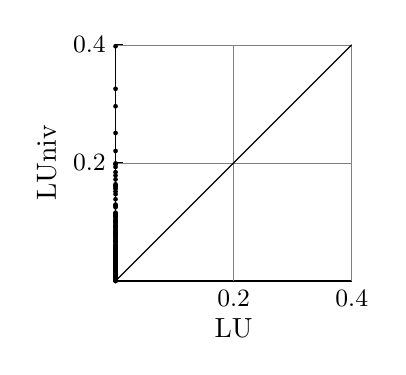
\begin{tikzpicture}

\draw (0,0) -- (3,0);
\node at (1.5,-0.6) {LU};
\node [anchor=north] at (1.5,0) {\small 0.2};
\draw (1.5,0) -- (1.5,0.1);
\draw [style=help lines] (1.5,0) -- (1.5,3);
\node [anchor=north] at (3,0) {\small 0.4};
\draw (3,0) -- (3,0.1);
\draw [style=help lines] (3,0) -- (3,3);
\draw (0,0) -- (0,3);
\node [rotate=90] at (-2.5em,1.5) {LUniv};
\node [anchor=east] at (0,1.499) {\small 0.2};
\draw (0,1.499) -- (0.1,1.499);
\draw [style=help lines] (0,1.499) -- (3,1.499);
\node [anchor=east] at (0,2.998) {\small 0.4};
\draw (0,2.998) -- (0.1,2.998);
\draw [style=help lines] (0,2.998) -- (3,2.998);
\foreach \pos in {
	(0.000000, 0.000000),
	(0.000000, 0.006027),
	(0.000000, 0.012068),
	(0.000000, 0.018078),
	(0.000000, 0.024081),
	(0.000000, 0.030102),
	(0.000000, 0.036132),
	(0.000000, 0.042135),
	(0.000000, 0.048139),
	(0.000000, 0.054173),
	(0.000000, 0.060193),
	(0.000000, 0.066204),
	(0.000000, 0.072231),
	(0.000000, 0.078267),
	(0.000000, 0.084364),
	(0.000000, 0.090399),
	(0.000000, 0.096401),
	(0.000000, 0.102428),
	(0.000000, 0.108447),
	(0.000000, 0.114679),
	(0.000000, 0.120791),
	(0.000000, 0.126880),
	(0.000000, 0.132911),
	(0.000000, 0.139104),
	(0.000000, 0.145161),
	(0.000000, 0.151976),
	(0.000000, 0.158056),
	(0.000000, 0.164294),
	(0.000000, 0.170607),
	(0.000000, 0.177083),
	(0.000000, 0.183346),
	(0.000000, 0.189531),
	(0.000000, 0.197023),
	(0.000000, 0.203202),
	(0.000000, 0.210068),
	(0.000000, 0.216346),
	(0.000000, 0.222534),
	(0.000000, 0.228814),
	(0.000000, 0.235149),
	(0.000000, 0.242236),
	(0.000000, 0.248494),
	(0.000000, 0.255682),
	(0.000000, 0.262190),
	(0.000000, 0.268595),
	(0.000000, 0.275000),
	(0.000000, 0.281250),
	(0.000000, 0.288652),
	(0.000000, 0.295468),
	(0.000000, 0.302469),
	(0.000000, 0.309633),
	(0.000000, 0.317199),
	(0.000000, 0.323920),
	(0.000000, 0.330264),
	(0.000000, 0.337955),
	(0.000000, 0.343960),
	(0.000000, 0.353213),
	(0.000000, 0.359281),
	(0.000000, 0.367948),
	(0.000000, 0.376227),
	(0.000000, 0.382883),
	(0.000000, 0.389447),
	(0.000000, 0.396635),
	(0.000000, 0.403226),
	(0.000000, 0.410584),
	(0.000000, 0.418424),
	(0.000000, 0.425226),
	(0.000000, 0.432000),
	(0.000000, 0.442446),
	(0.000000, 0.449183),
	(0.000000, 0.456933),
	(0.000000, 0.468750),
	(0.000000, 0.489614),
	(0.000000, 0.500000),
	(0.000000, 0.507201),
	(0.000000, 0.513219),
	(0.000000, 0.520112),
	(0.000000, 0.535714),
	(0.000000, 0.552826),
	(0.000000, 0.566406),
	(0.000000, 0.573940),
	(0.000000, 0.582320),
	(0.000000, 0.591603),
	(0.000000, 0.603998),
	(0.000000, 0.610329),
	(0.000000, 0.617089),
	(0.000000, 0.629845),
	(0.000000, 0.645161),
	(0.000000, 0.659843),
	(0.000000, 0.680628),
	(0.000000, 0.689189),
	(0.000000, 0.696653),
	(0.000000, 0.703125),
	(0.000000, 0.722940),
	(0.000000, 0.738137),
	(0.000000, 0.750000),
	(0.000000, 0.756961),
	(0.000000, 0.765571),
	(0.000000, 0.772382),
	(0.000000, 0.796943),
	(0.000000, 0.814917),
	(0.000000, 0.825147),
	(0.000000, 0.833333),
	(0.000000, 0.843426),
	(0.000000, 0.853716),
	(0.000000, 0.867993),
	(0.000000, 0.936396),
	(0.000000, 0.953237),
	(0.000000, 0.961538),
	(0.000000, 0.970588),
	(0.000000, 1.038405),
	(0.000000, 1.102151),
	(0.000000, 1.135487),
	(0.000000, 1.169637),
	(0.000000, 1.192255),
	(0.000000, 1.207154),
	(0.000000, 1.214489),
	(0.000000, 1.228771),
	(0.000000, 1.289409),
	(0.000000, 1.338120),
	(0.000000, 1.382175),
	(0.000000, 1.447721),
	(0.000000, 1.481127),
	(0.000000, 1.493478),
	(0.000000, 1.651376),
	(0.000000, 1.879845),
	(0.000000, 2.219101),
	(0.000000, 2.440727),
	(0.000000, 2.981462),
} \fill \pos circle(0.03);
\draw (0,0) -- (3, 3);
\end{tikzpicture}

  } \
  \subfloat[Compression ratio difference]{
    \centering
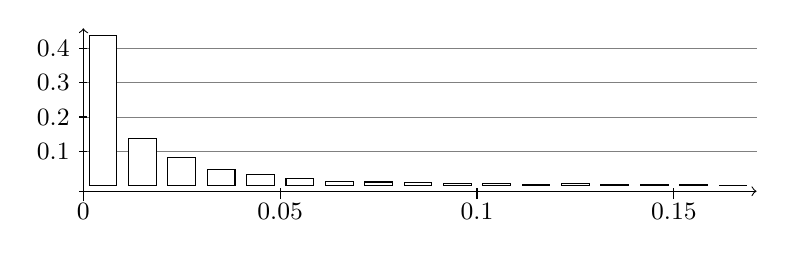
\begin{tikzpicture}
\draw[->] (-0.25,-0.2) -- (-0.25,2);
\draw [style=help lines] (-0.3,0.436406513976431) -- (8.3,0.436406513976431);
\node [anchor=east,fill=white] at (-0.3,0.436406513976431) {\small 0.1};
\draw (-0.3,0.436406513976431) -- (-0.2,0.436406513976431);
\draw [style=help lines] (-0.3,0.872813027952862) -- (8.3,0.872813027952862);
\node [anchor=east,fill=white] at (-0.3,0.872813027952862) {\small 0.2};
\draw (-0.3,0.872813027952862) -- (-0.2,0.872813027952862);
\draw [style=help lines] (-0.3,1.30921954192929) -- (8.3,1.30921954192929);
\node [anchor=east,fill=white] at (-0.3,1.30921954192929) {\small 0.3};
\draw (-0.3,1.30921954192929) -- (-0.2,1.30921954192929);
\draw [style=help lines] (-0.3,1.74562605590572) -- (8.3,1.74562605590572);
\node [anchor=east,fill=white] at (-0.3,1.74562605590572) {\small 0.4};
\draw (-0.3,1.74562605590572) -- (-0.2,1.74562605590572);
\draw[->] (-0.3,-0.07) -- (8.3,-0.07);
\node [anchor=north] at (-0.25, -0.1) {\small 0};
\draw (-0.25,-0.17) -- (-0.25,-0.03);
\node [anchor=north] at (2.25, -0.1) {\small 0.05};
\draw (2.25,-0.17) -- (2.25,-0.03);
\node [anchor=north] at (4.75, -0.1) {\small 0.1};
\draw (4.75,-0.17) -- (4.75,-0.03);
\node [anchor=north] at (7.25, -0.1) {\small 0.15};
\draw (7.25,-0.17) -- (7.25,-0.03);

\draw[fill=white] plot[ybar] coordinates {
	(6.000000, 0.027668)
	(6.500000, 0.011240)
	(7.500000, 0.014698)
	(3.000000, 0.054470)
	(5.500000, 0.014698)
	(5.000000, 0.025074)
	(8.000000, 0.005188)
	(1.500000, 0.202319)
	(4.500000, 0.032855)
	(3.500000, 0.046689)
	(0.500000, 0.601769)
	(0.000000, 1.912519)
	(4.000000, 0.044960)
	(2.500000, 0.094243)
	(1.000000, 0.361407)
	(2.000000, 0.138338)
	(7.000000, 0.012969)
};

\end{tikzpicture}
  } \
  \subfloat[Duration difference]{
    \centering
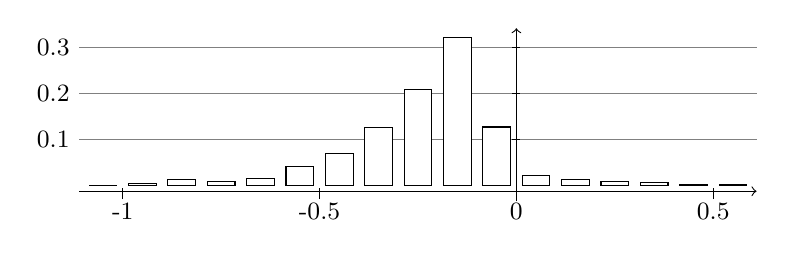
\begin{tikzpicture}
\draw[->] (-0.25,-0.2) -- (-0.25,2);
\draw [style=help lines] (-5.8,0.585829681355775) -- (2.8,0.585829681355775);
\node [anchor=east,fill=white] at (-5.8,0.585829681355775) {\small 0.1};
\draw (-0.3,0.585829681355775) -- (-0.2,0.585829681355775);
\draw [style=help lines] (-5.8,1.17165936271155) -- (2.8,1.17165936271155);
\node [anchor=east,fill=white] at (-5.8,1.17165936271155) {\small 0.2};
\draw (-0.3,1.17165936271155) -- (-0.2,1.17165936271155);
\draw [style=help lines] (-5.8,1.75748904406732) -- (2.8,1.75748904406732);
\node [anchor=east,fill=white] at (-5.8,1.75748904406732) {\small 0.3};
\draw (-0.3,1.75748904406732) -- (-0.2,1.75748904406732);
\draw[->] (-5.8,-0.07) -- (2.8,-0.07);
\node [anchor=north] at (-5.25, -0.1) {\small -1};
\draw (-5.25,-0.17) -- (-5.25,-0.03);
\node [anchor=north] at (-2.75, -0.1) {\small -0.5};
\draw (-2.75,-0.17) -- (-2.75,-0.03);
\node [anchor=north] at (-0.25, -0.1) {\small 0};
\draw (-0.25,-0.17) -- (-0.25,-0.03);
\node [anchor=north] at (2.25, -0.1) {\small 0.5};
\draw (2.25,-0.17) -- (2.25,-0.03);

\draw[fill=white] plot[ybar] coordinates {
	(1.000000, 0.048719)
	(-4.000000, 0.054519)
	(1.500000, 0.041759)
	(-4.500000, 0.077718)
	(0.000000, 0.132237)
	(-5.500000, 0.008120)
	(2.000000, 0.019720)
	(-3.500000, 0.092798)
	(0.500000, 0.080038)
	(-0.500000, 0.745862)
	(-3.000000, 0.249394)
	(-2.000000, 0.741222)
	(-1.000000, 1.882634)
	(2.500000, 0.015080)
	(-1.500000, 1.223770)
	(-5.000000, 0.025519)
	(-2.500000, 0.409470)
};

\end{tikzpicture}
  }
  \caption{Comparison between LU and LUniv}
  \label{fig:LU}
\end{figure}


As expected, {\LowerUnivalents} always compresses more than {\LowerUnits} (subfigure (a)) at the expense of a longer
computation (subfigure (d)). And even if the compression gain is low on average (as noticeable in Table \ref{tab:average}), subfigure (a) shows that {\LowerUnivalents} compresses some proofs significantly more than {\LowerUnits}.

It has to be noticed that \veriT already does its best to produce compact proofs. In particular,
a forward subsumption algorithm is applied, which results in proofs not having two different subproofs
with the same conclusion. This results in {\LowerUnits} being unable to reduce unsat core.
But as {\LowerUnivalents} lowers non-unit subproofs and performs some partial regularization, it
achieves some unsat core reduction, as noticeable in subfigure (b).

The comparison of the sequential \texttt{LU.RPI} with the non-sequential {\LUnivRPI} shown in Fig.
\ref{fig:LUnivRPI} outlines the ability of {\LowerUnivalents} to be efficiently combined with other
algorithms. Not only compression ratios are improved but {\LUnivRPI} is faster than the sequential
composition for more than 80 \% of the proofs.



\begin{figure}[tb]
  \centering
  \subfloat[Compression ratio]{
    \centering
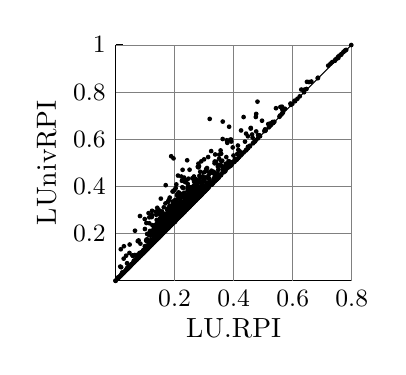
\begin{tikzpicture}

\draw (0,0) -- (3,0);
\node at (1.5,-0.6) {LU.RPI};
\node [anchor=north] at (0.75,0) {\small 0.2};
\draw (0.75,0) -- (0.75,0.1);
\draw [style=help lines] (0.75,0) -- (0.75,3);
\node [anchor=north] at (1.5,0) {\small 0.4};
\draw (1.5,0) -- (1.5,0.1);
\draw [style=help lines] (1.5,0) -- (1.5,3);
\node [anchor=north] at (2.25,0) {\small 0.6};
\draw (2.25,0) -- (2.25,0.1);
\draw [style=help lines] (2.25,0) -- (2.25,3);
\node [anchor=north] at (3,0) {\small 0.8};
\draw (3,0) -- (3,0.1);
\draw [style=help lines] (3,0) -- (3,3);
\draw (0,0) -- (0,3);
\node [rotate=90] at (-2.5em,1.5) {LUnivRPI};
\node [anchor=east] at (0,0.599) {\small 0.2};
\draw (0,0.599) -- (0.1,0.599);
\draw [style=help lines] (0,0.599) -- (3,0.599);
\node [anchor=east] at (0,1.198) {\small 0.4};
\draw (0,1.198) -- (0.1,1.198);
\draw [style=help lines] (0,1.198) -- (3,1.198);
\node [anchor=east] at (0,1.797) {\small 0.6};
\draw (0,1.797) -- (0.1,1.797);
\draw [style=help lines] (0,1.797) -- (3,1.797);
\node [anchor=east] at (0,2.396) {\small 0.8};
\draw (0,2.396) -- (0.1,2.396);
\draw [style=help lines] (0,2.396) -- (3,2.396);
\node [anchor=east] at (0,2.995) {\small 1};
\draw (0,2.995) -- (0.1,2.995);
\draw [style=help lines] (0,2.995) -- (3,2.995);
\foreach \pos in {
	(0.000000, 0.000000),
	(0.022556, 0.022556),
	(0.026866, 0.026866),
	(0.034884, 0.034884),
	(0.033771, 0.044224),
	(0.039735, 0.039735),
	(0.047782, 0.047782),
	(0.055046, 0.055046),
	(0.061529, 0.061529),
	(0.065990, 0.065990),
	(0.071429, 0.071429),
	(0.075949, 0.075949),
	(0.078947, 0.086842),
	(0.086185, 0.086185),
	(0.092593, 0.092593),
	(0.084806, 0.106007),
	(0.099919, 0.099919),
	(0.104966, 0.104966),
	(0.110092, 0.110092),
	(0.114504, 0.114504),
	(0.122041, 0.122041),
	(0.128571, 0.128571),
	(0.071303, 0.171655),
	(0.060000, 0.180000),
	(0.136364, 0.136364),
	(0.142012, 0.142012),
	(0.141340, 0.149701),
	(0.146341, 0.146341),
	(0.151899, 0.151899),
	(0.156780, 0.156780),
	(0.150729, 0.170178),
	(0.162712, 0.162712),
	(0.168000, 0.168000),
	(0.173077, 0.173077),
	(0.177515, 0.177515),
	(0.182657, 0.182657),
	(0.145941, 0.222798),
	(0.190909, 0.190909),
	(0.195918, 0.195918),
	(0.204545, 0.204545),
	(0.200856, 0.210782),
	(0.103448, 0.280788),
	(0.211973, 0.214269),
	(0.221051, 0.221549),
	(0.225348, 0.228804),
	(0.233010, 0.233010),
	(0.238054, 0.238805),
	(0.231502, 0.252513),
	(0.241615, 0.244870),
	(0.134328, 0.318408),
	(0.248121, 0.248730),
	(0.242163, 0.256984),
	(0.252074, 0.257542),
	(0.258219, 0.258427),
	(0.252366, 0.264420),
	(0.259315, 0.265075),
	(0.265513, 0.265513),
	(0.269674, 0.269879),
	(0.222026, 0.314537),
	(0.268906, 0.276229),
	(0.214286, 0.321429),
	(0.275511, 0.275726),
	(0.270148, 0.283768),
	(0.176471, 0.352941),
	(0.279610, 0.281561),
	(0.066667, 0.400000),
	(0.286393, 0.287182),
	(0.244898, 0.326531),
	(0.285177, 0.295294),
	(0.291667, 0.291667),
	(0.296928, 0.296928),
	(0.300130, 0.302734),
	(0.307058, 0.307831),
	(0.302600, 0.313489),
	(0.284211, 0.331579),
	(0.301693, 0.320207),
	(0.311584, 0.311792),
	(0.310383, 0.317737),
	(0.316484, 0.316484),
	(0.106195, 0.438053),
	(0.313074, 0.324653),
	(0.320626, 0.322031),
	(0.325434, 0.326011),
	(0.318974, 0.334808),
	(0.315469, 0.341907),
	(0.326271, 0.332227),
	(0.305505, 0.353670),
	(0.332547, 0.332547),
	(0.324825, 0.343055),
	(0.334427, 0.339516),
	(0.333588, 0.346735),
	(0.340909, 0.340909),
	(0.329980, 0.357339),
	(0.339402, 0.348831),
	(0.345455, 0.345455),
	(0.332109, 0.364030),
	(0.179221, 0.459740),
	(0.345945, 0.353188),
	(0.351792, 0.351792),
	(0.348837, 0.358804),
	(0.356265, 0.356512),
	(0.355974, 0.364317),
	(0.360921, 0.360921),
	(0.346738, 0.375993),
	(0.366084, 0.366105),
	(0.361655, 0.370806),
	(0.360262, 0.377479),
	(0.370662, 0.370684),
	(0.367135, 0.378819),
	(0.355440, 0.392429),
	(0.364115, 0.385163),
	(0.374950, 0.374988),
	(0.372969, 0.382027),
	(0.379331, 0.379521),
	(0.369434, 0.391811),
	(0.376535, 0.388813),
	(0.383470, 0.384334),
	(0.381187, 0.393701),
	(0.388263, 0.388556),
	(0.381963, 0.401857),
	(0.392587, 0.392718),
	(0.389875, 0.398283),
	(0.388031, 0.404186),
	(0.396528, 0.397336),
	(0.380041, 0.416875),
	(0.395580, 0.403315),
	(0.315881, 0.471023),
	(0.401438, 0.401541),
	(0.391266, 0.417037),
	(0.400591, 0.410781),
	(0.405797, 0.405797),
	(0.371866, 0.438719),
	(0.282110, 0.502294),
	(0.393529, 0.422730),
	(0.405007, 0.414862),
	(0.410853, 0.410853),
	(0.399240, 0.424905),
	(0.392027, 0.433555),
	(0.405433, 0.422848),
	(0.412802, 0.417751),
	(0.292683, 0.512195),
	(0.402659, 0.435226),
	(0.419692, 0.419692),
	(0.421184, 0.425797),
	(0.427612, 0.427734),
	(0.423215, 0.435209),
	(0.415609, 0.443377),
	(0.429151, 0.434300),
	(0.423256, 0.445349),
	(0.435256, 0.435368),
	(0.432916, 0.441732),
	(0.424676, 0.454307),
	(0.439511, 0.441052),
	(0.430712, 0.453184),
	(0.439107, 0.449259),
	(0.444795, 0.444795),
	(0.426309, 0.467243),
	(0.447369, 0.450247),
	(0.440077, 0.458763),
	(0.435583, 0.463190),
	(0.397732, 0.498631),
	(0.451080, 0.455735),
	(0.445668, 0.461316),
	(0.389262, 0.510067),
	(0.457061, 0.457419),
	(0.434292, 0.480493),
	(0.451189, 0.467641),
	(0.442037, 0.476676),
	(0.456647, 0.463621),
	(0.462555, 0.462555),
	(0.393516, 0.523691),
	(0.430969, 0.496568),
	(0.453807, 0.478173),
	(0.463568, 0.469922),
	(0.459797, 0.476456),
	(0.407631, 0.524096),
	(0.469785, 0.470615),
	(0.454803, 0.488338),
	(0.473595, 0.475379),
	(0.468025, 0.481294),
	(0.458019, 0.495482),
	(0.478819, 0.478960),
	(0.466975, 0.490559),
	(0.247059, 0.635294),
	(0.476424, 0.489682),
	(0.482688, 0.483707),
	(0.449591, 0.514986),
	(0.462162, 0.510811),
	(0.484317, 0.490023),
	(0.469266, 0.506422),
	(0.476190, 0.503401),
	(0.483945, 0.496157),
	(0.490444, 0.491278),
	(0.491765, 0.497793),
	(0.483823, 0.510249),
	(0.497727, 0.498605),
	(0.481799, 0.517131),
	(0.473310, 0.528146),
	(0.491691, 0.512664),
	(0.502547, 0.502744),
	(0.497695, 0.509062),
	(0.492667, 0.520186),
	(0.503893, 0.509530),
	(0.401709, 0.593831),
	(0.500591, 0.516054),
	(0.421813, 0.583443),
	(0.492559, 0.526590),
	(0.498788, 0.522055),
	(0.509770, 0.511427),
	(0.441951, 0.573659),
	(0.505588, 0.520140),
	(0.496173, 0.531888),
	(0.485763, 0.542180),
	(0.514151, 0.516221),
	(0.502830, 0.528835),
	(0.417722, 0.600000),
	(0.497124, 0.539432),
	(0.511285, 0.526364),
	(0.519434, 0.519518),
	(0.509844, 0.532426),
	(0.505670, 0.536929),
	(0.521818, 0.525696),
	(0.500000, 0.547297),
	(0.516432, 0.533646),
	(0.523554, 0.531853),
	(0.529006, 0.529195),
	(0.520112, 0.541093),
	(0.510104, 0.552888),
	(0.479666, 0.579944),
	(0.525795, 0.538924),
	(0.530846, 0.535292),
	(0.373010, 0.657316),
	(0.536817, 0.536817),
	(0.529679, 0.544022),
	(0.522862, 0.550834),
	(0.464343, 0.607429),
	(0.529143, 0.552029),
	(0.540770, 0.541800),
	(0.537037, 0.549383),
	(0.439024, 0.633208),
	(0.517061, 0.572528),
	(0.529363, 0.561219),
	(0.545306, 0.545851),
	(0.542941, 0.551788),
	(0.539863, 0.559226),
	(0.549707, 0.550018),
	(0.537190, 0.566116),
	(0.529698, 0.573515),
	(0.518506, 0.584720),
	(0.547740, 0.557584),
	(0.554702, 0.554702),
	(0.544983, 0.564446),
	(0.536177, 0.575181),
	(0.470004, 0.631404),
	(0.520354, 0.593363),
	(0.550684, 0.566530),
	(0.557879, 0.560014),
	(0.488646, 0.622150),
	(0.545502, 0.574295),
	(0.557056, 0.569210),
	(0.563150, 0.563276),
	(0.550360, 0.578237),
	(0.534542, 0.593023),
	(0.528352, 0.602062),
	(0.564607, 0.569443),
	(0.493103, 0.636782),
	(0.501548, 0.631579),
	(0.570848, 0.571033),
	(0.555000, 0.587857),
	(0.559933, 0.583657),
	(0.565851, 0.578345),
	(0.540089, 0.607969),
	(0.574954, 0.575646),
	(0.556161, 0.595420),
	(0.568569, 0.585179),
	(0.549451, 0.604396),
	(0.578765, 0.580405),
	(0.484605, 0.662651),
	(0.563822, 0.598104),
	(0.523636, 0.635455),
	(0.535851, 0.625717),
	(0.576655, 0.588464),
	(0.561896, 0.604462),
	(0.584743, 0.584743),
	(0.576630, 0.595498),
	(0.559254, 0.613182),
	(0.568398, 0.604883),
	(0.548929, 0.623625),
	(0.391560, 0.733072),
	(0.584871, 0.591158),
	(0.575703, 0.603696),
	(0.507763, 0.662100),
	(0.585389, 0.597674),
	(0.591887, 0.592359),
	(0.578804, 0.611413),
	(0.587723, 0.603244),
	(0.594961, 0.597991),
	(0.576445, 0.617501),
	(0.546099, 0.645390),
	(0.586176, 0.609515),
	(0.429007, 0.729997),
	(0.468547, 0.706074),
	(0.594006, 0.606043),
	(0.572968, 0.626644),
	(0.599106, 0.602735),
	(0.564000, 0.636000),
	(0.570608, 0.634647),
	(0.585509, 0.622715),
	(0.598271, 0.610833),
	(0.545997, 0.659373),
	(0.604267, 0.606442),
	(0.581081, 0.632883),
	(0.573620, 0.640412),
	(0.565923, 0.648073),
	(0.597603, 0.619472),
	(0.587071, 0.630607),
	(0.603268, 0.615260),
	(0.592888, 0.626505),
	(0.609664, 0.610784),
	(0.556808, 0.660885),
	(0.582822, 0.639264),
	(0.599952, 0.624997),
	(0.573326, 0.649538),
	(0.370787, 0.783708),
	(0.609045, 0.617268),
	(0.590614, 0.636554),
	(0.508787, 0.703866),
	(0.566809, 0.658723),
	(0.546019, 0.676319),
	(0.615541, 0.616339),
	(0.576191, 0.655027),
	(0.600816, 0.632653),
	(0.609176, 0.625043),
	(0.562297, 0.669556),
	(0.585000, 0.650000),
	(0.509510, 0.711224),
	(0.593318, 0.644098),
	(0.615639, 0.622825),
	(0.542510, 0.688259),
	(0.310345, 0.821839),
	(0.614063, 0.629464),
	(0.621995, 0.622704),
	(0.564644, 0.675462),
	(0.611009, 0.638532),
	(0.604077, 0.647931),
	(0.620371, 0.632567),
	(0.589699, 0.661359),
	(0.625328, 0.628383),
	(0.556856, 0.689799),
	(0.578740, 0.671915),
	(0.533173, 0.709522),
	(0.617043, 0.638604),
	(0.600000, 0.660502),
	(0.626232, 0.637315),
	(0.632022, 0.632748),
	(0.524272, 0.724919),
	(0.591534, 0.673016),
	(0.600467, 0.668638),
	(0.622877, 0.648033),
	(0.628127, 0.643134),
	(0.634298, 0.638813),
	(0.615904, 0.658767),
	(0.600000, 0.675000),
	(0.606099, 0.670902),
	(0.640281, 0.640691),
	(0.634599, 0.646769),
	(0.628846, 0.653159),
	(0.624590, 0.657787),
	(0.568508, 0.707735),
	(0.580034, 0.700516),
	(0.586466, 0.696026),
	(0.619637, 0.666933),
	(0.612762, 0.673381),
	(0.641038, 0.647636),
	(0.636210, 0.652868),
	(0.428571, 0.805132),
	(0.604142, 0.685584),
	(0.628272, 0.665766),
	(0.621106, 0.673367),
	(0.642096, 0.654123),
	(0.646739, 0.649954),
	(0.614955, 0.680804),
	(0.564516, 0.725806),
	(0.637981, 0.664236),
	(0.622199, 0.681605),
	(0.650591, 0.654940),
	(0.604580, 0.698931),
	(0.585600, 0.715200),
	(0.646423, 0.661398),
	(0.610417, 0.695833),
	(0.629728, 0.679275),
	(0.637287, 0.672988),
	(0.581315, 0.722491),
	(0.450673, 0.810538),
	(0.644534, 0.669809),
	(0.656579, 0.658198),
	(0.652430, 0.662739),
	(0.577845, 0.730080),
	(0.608434, 0.704819),
	(0.460317, 0.809524),
	(0.522321, 0.772321),
	(0.624582, 0.692308),
	(0.637964, 0.680780),
	(0.631579, 0.687673),
	(0.560786, 0.747258),
	(0.643736, 0.677870),
	(0.593318, 0.722940),
	(0.653666, 0.669501),
	(0.661269, 0.662350),
	(0.649566, 0.674162),
	(0.574523, 0.740901),
	(0.660618, 0.668743),
	(0.643099, 0.685972),
	(0.656688, 0.674930),
	(0.649706, 0.683872),
	(0.666667, 0.668519),
	(0.605181, 0.725275),
	(0.622695, 0.710511),
	(0.591488, 0.737723),
	(0.663555, 0.674274),
	(0.637902, 0.699662),
	(0.643500, 0.696750),
	(0.617747, 0.720137),
	(0.649499, 0.691887),
	(0.656291, 0.685489),
	(0.671732, 0.671791),
	(0.669326, 0.677714),
	(0.631854, 0.712794),
	(0.613890, 0.730467),
	(0.462527, 0.835118),
	(0.666184, 0.684095),
	(0.419355, 0.858871),
	(0.660603, 0.690761),
	(0.675292, 0.676972),
	(0.628440, 0.723394),
	(0.643590, 0.710876),
	(0.672229, 0.684224),
	(0.653345, 0.702867),
	(0.622140, 0.731121),
	(0.668372, 0.690233),
	(0.660365, 0.699210),
	(0.680638, 0.680638),
	(0.651363, 0.709355),
	(0.667491, 0.696490),
	(0.676734, 0.688607),
	(0.619124, 0.741036),
	(0.579987, 0.772154),
	(0.561447, 0.786026),
	(0.673967, 0.694356),
	(0.663454, 0.705653),
	(0.682847, 0.688796),
	(0.660585, 0.711498),
	(0.670562, 0.703433),
	(0.641260, 0.730488),
	(0.680286, 0.695778),
	(0.628086, 0.745474),
	(0.688761, 0.689821),
	(0.670355, 0.710638),
	(0.677700, 0.704518),
	(0.663000, 0.718500),
	(0.685052, 0.701381),
	(0.691047, 0.695599),
	(0.656683, 0.728404),
	(0.676932, 0.711125),
	(0.670711, 0.717269),
	(0.516673, 0.837669),
	(0.684158, 0.707921),
	(0.632212, 0.754808),
	(0.666667, 0.725074),
	(0.655629, 0.735099),
	(0.690789, 0.703205),
	(0.696795, 0.697788),
	(0.585000, 0.795000),
	(0.601744, 0.784884),
	(0.698192, 0.704061),
	(0.687540, 0.715279),
	(0.677248, 0.725085),
	(0.595916, 0.794554),
	(0.647197, 0.753742),
	(0.661702, 0.741162),
	(0.695178, 0.711721),
	(0.685511, 0.722587),
	(0.634398, 0.768280),
	(0.639537, 0.764626),
	(0.701914, 0.709410),
	(0.692243, 0.721331),
	(0.672467, 0.740020),
	(0.617111, 0.788219),
	(0.667333, 0.746549),
	(0.707872, 0.708476),
	(0.679007, 0.736222),
	(0.688236, 0.728005),
	(0.463520, 0.888185),
	(0.684329, 0.732824),
	(0.698323, 0.720509),
	(0.703722, 0.716146),
	(0.655558, 0.763165),
	(0.612200, 0.799564),
	(0.569992, 0.830378),
	(0.710780, 0.715610),
	(0.693350, 0.732871),
	(0.704622, 0.722703),
	(0.666290, 0.759828),
	(0.673236, 0.755245),
	(0.648719, 0.776775),
	(0.703671, 0.729185),
	(0.712065, 0.722339),
	(0.697936, 0.737336),
	(0.510245, 0.877917),
	(0.679634, 0.755835),
	(0.718264, 0.719546),
	(0.688536, 0.748468),
	(0.541907, 0.862479),
	(0.711564, 0.729999),
	(0.666401, 0.771497),
	(0.706723, 0.735310),
	(0.717212, 0.726716),
	(0.697500, 0.747500),
	(0.662409, 0.779562),
	(0.704826, 0.741900),
	(0.693477, 0.753305),
	(0.713230, 0.736576),
	(0.723319, 0.728187),
	(0.646501, 0.798561),
	(0.653531, 0.793416),
	(0.719399, 0.734431),
	(0.636953, 0.807131),
	(0.668405, 0.782414),
	(0.705277, 0.749387),
	(0.700897, 0.754709),
	(0.679426, 0.775120),
	(0.692854, 0.763916),
	(0.729127, 0.729710),
	(0.605948, 0.837361),
	(0.726049, 0.735930),
	(0.719982, 0.742152),
	(0.711864, 0.750934),
	(0.661538, 0.796154),
	(0.689420, 0.773281),
	(0.701099, 0.762805),
	(0.654944, 0.805242),
	(0.634301, 0.822142),
	(0.719828, 0.748922),
	(0.732082, 0.737305),
	(0.710153, 0.759074),
	(0.695481, 0.772543),
	(0.725632, 0.744585),
	(0.676320, 0.790689),
	(0.715920, 0.756168),
	(0.685349, 0.786651),
	(0.733915, 0.743184),
	(0.730391, 0.748385),
	(0.667355, 0.806026),
	(0.589641, 0.864542),
	(0.723855, 0.756664),
	(0.714837, 0.765194),
	(0.677005, 0.799572),
	(0.569826, 0.879440),
	(0.741053, 0.742176),
	(0.698537, 0.782439),
	(0.737185, 0.749359),
	(0.730241, 0.756586),
	(0.713836, 0.772537),
	(0.722222, 0.766667),
	(0.691682, 0.795848),
	(0.745814, 0.746014),
	(0.736735, 0.755685),
	(0.545735, 0.903392),
	(0.712220, 0.779365),
	(0.731443, 0.764387),
	(0.719450, 0.775787),
	(0.628713, 0.851485),
	(0.752504, 0.745351),
	(0.658188, 0.829889),
	(0.653114, 0.833901),
	(0.589286, 0.880309),
	(0.745298, 0.753858),
	(0.740913, 0.760485),
	(0.727334, 0.773932),
	(0.717965, 0.783791),
	(0.684952, 0.813128),
	(0.677342, 0.821457),
	(0.737080, 0.769073),
	(0.752855, 0.754345),
	(0.747506, 0.762013),
	(0.529625, 0.926844),
	(0.742829, 0.767214),
	(0.731650, 0.779006),
	(0.716727, 0.793385),
	(0.700855, 0.809117),
	(0.695017, 0.815046),
	(0.755359, 0.760519),
	(0.748395, 0.769489),
	(0.682175, 0.829587),
	(0.727246, 0.790754),
	(0.720415, 0.798157),
	(0.732510, 0.787380),
	(0.695531, 0.821229),
	(0.761719, 0.761719),
	(0.743410, 0.780264),
	(0.755990, 0.768397),
	(0.749288, 0.776353),
	(0.716005, 0.808208),
	(0.689072, 0.832689),
	(0.679669, 0.840574),
	(0.712500, 0.813281),
	(0.701964, 0.822508),
	(0.763443, 0.767710),
	(0.663889, 0.855556),
	(0.745673, 0.787058),
	(0.759090, 0.774591),
	(0.730271, 0.803116),
	(0.719383, 0.814065),
	(0.755293, 0.781614),
	(0.716692, 0.820061),
	(0.770690, 0.770690),
	(0.765752, 0.776330),
	(0.750000, 0.792339),
	(0.761941, 0.781766),
	(0.711746, 0.828203),
	(0.743503, 0.800000),
	(0.736919, 0.807776),
	(0.690962, 0.847522),
	(0.759612, 0.787573),
	(0.703877, 0.838235),
	(0.752134, 0.797977),
	(0.768352, 0.782423),
	(0.680707, 0.860054),
	(0.773592, 0.777800),
	(0.712261, 0.836311),
	(0.766092, 0.788252),
	(0.719057, 0.834971),
	(0.775215, 0.783655),
	(0.760090, 0.798694),
	(0.740310, 0.817829),
	(0.756032, 0.804290),
	(0.748544, 0.812621),
	(0.771443, 0.791078),
	(0.766607, 0.797149),
	(0.781686, 0.783581),
	(0.746939, 0.818878),
	(0.765415, 0.803234),
	(0.777372, 0.792492),
	(0.755097, 0.813846),
	(0.773864, 0.797727),
	(0.785974, 0.788430),
	(0.655539, 0.901366),
	(0.745161, 0.830323),
	(0.612552, 0.932528),
	(0.752003, 0.824387),
	(0.667042, 0.895388),
	(0.781806, 0.798802),
	(0.673901, 0.892324),
	(0.769280, 0.812123),
	(0.762641, 0.819098),
	(0.776916, 0.806429),
	(0.788243, 0.796459),
	(0.783488, 0.804971),
	(0.740307, 0.845244),
	(0.686636, 0.889401),
	(0.776081, 0.812621),
	(0.760320, 0.827950),
	(0.723902, 0.860251),
	(0.676281, 0.898292),
	(0.752446, 0.836413),
	(0.736522, 0.851304),
	(0.769320, 0.822581),
	(0.793541, 0.799485),
	(0.758538, 0.834783),
	(0.782743, 0.812492),
	(0.789756, 0.805837),
	(0.766946, 0.828452),
	(0.743195, 0.851251),
	(0.729794, 0.864105),
	(0.685665, 0.899827),
	(0.756303, 0.842174),
	(0.779279, 0.821922),
	(0.797406, 0.804794),
	(0.665476, 0.917857),
	(0.788634, 0.814670),
	(0.726562, 0.870536),
	(0.720643, 0.876391),
	(0.766905, 0.836463),
	(0.771681, 0.832610),
	(0.739572, 0.861497),
	(0.672671, 0.914907),
	(0.747226, 0.856350),
	(0.803742, 0.803906),
	(0.796925, 0.811321),
	(0.781915, 0.828191),
	(0.718127, 0.885516),
	(0.795444, 0.817599),
	(0.726901, 0.880551),
	(0.790971, 0.824062),
	(0.805315, 0.810602),
	(0.768365, 0.845797),
	(0.685448, 0.914622),
	(0.783784, 0.834719),
	(0.734115, 0.879349),
	(0.803759, 0.816661),
	(0.760829, 0.858571),
	(0.790482, 0.832145),
	(0.685934, 0.921002),
	(0.797017, 0.826848),
	(0.742698, 0.876596),
	(0.810193, 0.815343),
	(0.778365, 0.848306),
	(0.807780, 0.821442),
	(0.789641, 0.839030),
	(0.770155, 0.857259),
	(0.798701, 0.833079),
	(0.805171, 0.828255),
	(0.737643, 0.889734),
	(0.817518, 0.817518),
	(0.795068, 0.841959),
	(0.811087, 0.826661),
	(0.788985, 0.849370),
	(0.776724, 0.861318),
	(0.817366, 0.823863),
	(0.785443, 0.854699),
	(0.807268, 0.834232),
	(0.758602, 0.879847),
	(0.771593, 0.870304),
	(0.803714, 0.841228),
	(0.740764, 0.897828),
	(0.797900, 0.848644),
	(0.718232, 0.917127),
	(0.823412, 0.825324),
	(0.813662, 0.835982),
	(0.819174, 0.831425),
	(0.633627, 0.982356),
	(0.685069, 0.948557),
	(0.803307, 0.851416),
	(0.797526, 0.858014),
	(0.793062, 0.863475),
	(0.828531, 0.829556),
	(0.762326, 0.891277),
	(0.820397, 0.838164),
	(0.784149, 0.873711),
	(0.812191, 0.847948),
	(0.736986, 0.915068),
	(0.826704, 0.836351),
	(0.802029, 0.862078),
	(0.820010, 0.846003),
	(0.792307, 0.872060),
	(0.833333, 0.833333),
	(0.726841, 0.928741),
	(0.797967, 0.868617),
	(0.811892, 0.855863),
	(0.785081, 0.880543),
	(0.754135, 0.907903),
	(0.819079, 0.852418),
	(0.767694, 0.899439),
	(0.832350, 0.840080),
	(0.828667, 0.846053),
	(0.837987, 0.837987),
	(0.782983, 0.890057),
	(0.792653, 0.881616),
	(0.826393, 0.852409),
	(0.819486, 0.860825),
	(0.727067, 0.940430),
	(0.836393, 0.845172),
	(0.575385, 1.043077),
	(0.832663, 0.851971),
	(0.807692, 0.876244),
	(0.722054, 0.948640),
	(0.843263, 0.844408),
	(0.817591, 0.869343),
	(0.829926, 0.859287),
	(0.781863, 0.904638),
	(0.800730, 0.889980),
	(0.837404, 0.856306),
	(0.826198, 0.868371),
	(0.759116, 0.928177),
	(0.847135, 0.849730),
	(0.800099, 0.896229),
	(0.835699, 0.863656),
	(0.666786, 1.000718),
	(0.844348, 0.857575),
	(0.809672, 0.891120),
	(0.852272, 0.853398),
	(0.830852, 0.875744),
	(0.837015, 0.870148),
	(0.816016, 0.890139),
	(0.666833, 1.008492),
	(0.852095, 0.860172),
	(0.844291, 0.868977),
	(0.815109, 0.896543),
	(0.771299, 0.936416),
	(0.738592, 0.963380),
	(0.790733, 0.922902),
	(0.835438, 0.882891),
	(0.726354, 0.974640),
	(0.859717, 0.859949),
	(0.852205, 0.867867),
	(0.825727, 0.893621),
	(0.844675, 0.875801),
	(0.830769, 0.889718),
	(0.814206, 0.905047),
	(0.756522, 0.954037),
	(0.826138, 0.899650),
	(0.859010, 0.869109),
	(0.864238, 0.864238),
	(0.850903, 0.877384),
	(0.846560, 0.883142),
	(0.753233, 0.964170),
	(0.839432, 0.891089),
	(0.835474, 0.896715),
	(0.789634, 0.939024),
	(0.738386, 0.980440),
	(0.856913, 0.878858),
	(0.867594, 0.869941),
	(0.862375, 0.875694),
	(0.808989, 0.926966),
	(0.766491, 0.962527),
	(0.800960, 0.935654),
	(0.855366, 0.887494),
	(0.679567, 1.028742),
	(0.843976, 0.898945),
	(0.835995, 0.906514),
	(0.823688, 0.918945),
	(0.869136, 0.876543),
	(0.832595, 0.911866),
	(0.852615, 0.894966),
	(0.864639, 0.885630),
	(0.876246, 0.876246),
	(0.833703, 0.917823),
	(0.726064, 1.005319),
	(0.773781, 0.969881),
	(0.858359, 0.898429),
	(0.742748, 0.997710),
	(0.864124, 0.895171),
	(0.845124, 0.913660),
	(0.854105, 0.907023),
	(0.876621, 0.885399),
	(0.779549, 0.973081),
	(0.882249, 0.882544),
	(0.774444, 0.979307),
	(0.815476, 0.946429),
	(0.864307, 0.902655),
	(0.822434, 0.941317),
	(0.808412, 0.953735),
	(0.799927, 0.962326),
	(0.878003, 0.893095),
	(0.833107, 0.936228),
	(0.859507, 0.912824),
	(0.884972, 0.888653),
	(0.872123, 0.904038),
	(0.867658, 0.908618),
	(0.814205, 0.957124),
	(0.825133, 0.948319),
	(0.882709, 0.897326),
	(0.848735, 0.931793),
	(0.888543, 0.894672),
	(0.688679, 1.056604),
	(0.867640, 0.915815),
	(0.832285, 0.949161),
	(0.877278, 0.910308),
	(0.826817, 0.956864),
	(0.888577, 0.900904),
	(0.846510, 0.940787),
	(0.796236, 0.986088),
	(0.886070, 0.907241),
	(0.874576, 0.918644),
	(0.754720, 1.020875),
	(0.897022, 0.898883),
	(0.867135, 0.927823),
	(0.882597, 0.914685),
	(0.837828, 0.959913),
	(0.894769, 0.907158),
	(0.825176, 0.971622),
	(0.857028, 0.944177),
	(0.863116, 0.938974),
	(0.901963, 0.902349),
	(0.881197, 0.922652),
	(0.876364, 0.927879),
	(0.888043, 0.918335),
	(0.759825, 1.027293),
	(0.894570, 0.914723),
	(0.849595, 0.958964),
	(0.772702, 1.022014),
	(0.873278, 0.937611),
	(0.886649, 0.926162),
	(0.813071, 0.991831),
	(0.864382, 0.948359),
	(0.902947, 0.911879),
	(0.896050, 0.920891),
	(0.861226, 0.953706),
	(0.880961, 0.936162),
	(0.876522, 0.943602),
	(0.830447, 0.984751),
	(0.909155, 0.913760),
	(0.887076, 0.935626),
	(0.904283, 0.919380),
	(0.859554, 0.961979),
	(0.869005, 0.954263),
	(0.902157, 0.925133),
	(0.899661, 0.932021),
	(0.912559, 0.919806),
	(0.881214, 0.951996),
	(0.821842, 1.003702),
	(0.906635, 0.930711),
	(0.889027, 0.948878),
	(0.878439, 0.959754),
	(0.920522, 0.920681),
	(0.895837, 0.945412),
	(0.912844, 0.930275),
	(0.865385, 0.975962),
	(0.905430, 0.940045),
	(0.918696, 0.927155),
	(0.875087, 0.969209),
	(0.912332, 0.937432),
	(0.895696, 0.954846),
	(0.886838, 0.963884),
	(0.842135, 1.005741),
	(0.922233, 0.934270),
	(0.927792, 0.928813),
	(0.852545, 0.998402),
	(0.910633, 0.946380),
	(0.879971, 0.975192),
	(0.907781, 0.952450),
	(0.918374, 0.944151),
	(0.879410, 0.981398),
	(0.900402, 0.964716),
	(0.925898, 0.941940),
	(0.917570, 0.950108),
	(0.888685, 0.977303),
	(0.798165, 1.052752),
	(0.867351, 0.997069),
	(0.816955, 1.039100),
	(0.913379, 0.955772),
	(0.898831, 0.971903),
	(0.936548, 0.936548),
	(0.924197, 0.949036),
	(0.908441, 0.964235),
	(0.934385, 0.946950),
	(0.939553, 0.941974),
	(0.903131, 0.977129),
	(0.927783, 0.954009),
	(0.921659, 0.961598),
	(0.913119, 0.970043),
	(0.825320, 1.046414),
	(0.884778, 1.000000),
	(0.782450, 1.084095),
	(0.934835, 0.955828),
	(0.912584, 0.977324),
	(0.890380, 0.997763),
	(0.930026, 0.961872),
	(0.906975, 0.984004),
	(0.876581, 1.011339),
	(0.947368, 0.947368),
	(0.942578, 0.954650),
	(0.929099, 0.967955),
	(0.899836, 0.996716),
	(0.890168, 1.007218),
	(0.724341, 1.133580),
	(0.922958, 0.980740),
	(0.928636, 0.975610),
	(0.949709, 0.955678),
	(0.944774, 0.960749),
	(0.917946, 0.987524),
	(0.911232, 0.993890),
	(0.936704, 0.970726),
	(0.732907, 1.135946),
	(0.895477, 1.012931),
	(0.942718, 0.969903),
	(0.785941, 1.102574),
	(0.952672, 0.963724),
	(0.940425, 0.976972),
	(0.904242, 1.010667),
	(0.948772, 0.969991),
	(0.933962, 0.986097),
	(0.961965, 0.961980),
	(0.918182, 1.006061),
	(0.927236, 0.998131),
	(0.912423, 1.012113),
	(0.947030, 0.980202),
	(0.960529, 0.967888),
	(0.884828, 1.037824),
	(0.853345, 1.064688),
	(0.936433, 0.993359),
	(0.942857, 0.989204),
	(0.860868, 1.062904),
	(0.961832, 0.976251),
	(0.892528, 1.040590),
	(0.637209, 1.213953),
	(0.931275, 1.007495),
	(0.939717, 1.000775),
	(0.967768, 0.973737),
	(0.950923, 0.990199),
	(0.960726, 0.982880),
	(0.947215, 0.996108),
	(0.822586, 1.101931),
	(0.749035, 1.154440),
	(0.924212, 1.021872),
	(0.905206, 1.039677),
	(0.820612, 1.107710),
	(0.969894, 0.979735),
	(0.800135, 1.122916),
	(0.940496, 1.009096),
	(0.975877, 0.975877),
	(0.954348, 0.997205),
	(0.948519, 1.003469),
	(0.963449, 0.989462),
	(0.973752, 0.985375),
	(0.958177, 1.002289),
	(0.921896, 1.039591),
	(0.939249, 1.025460),
	(0.954390, 1.012324),
	(0.964705, 1.002667),
	(0.865155, 1.090229),
	(0.972208, 0.997640),
	(0.910922, 1.054497),
	(0.961789, 1.008388),
	(0.979878, 0.993917),
	(0.955010, 1.019264),
	(0.941893, 1.031733),
	(0.969964, 1.006613),
	(0.987623, 0.990340),
	(0.933549, 1.042139),
	(0.896766, 1.074251),
	(0.918512, 1.058189),
	(0.981826, 1.000606),
	(0.955192, 1.026282),
	(0.763975, 1.177019),
	(0.990070, 0.997471),
	(0.966117, 1.021978),
	(0.980049, 1.008943),
	(0.954873, 1.033354),
	(0.940157, 1.047469),
	(0.996301, 0.996521),
	(0.907174, 1.079490),
	(0.987425, 1.007186),
	(0.876276, 1.106824),
	(0.966133, 1.029369),
	(0.939538, 1.054509),
	(0.979372, 1.020269),
	(0.893339, 1.096430),
	(0.993639, 1.009404),
	(0.998823, 1.004474),
	(0.871249, 1.117377),
	(0.969437, 1.039258),
	(0.941806, 1.065429),
	(0.993137, 1.018531),
	(0.986210, 1.025451),
	(1.003945, 1.009864),
	(0.920327, 1.087845),
	(1.000000, 1.015802),
	(0.978042, 1.039373),
	(0.960915, 1.055291),
	(0.988661, 1.032756),
	(1.001526, 1.022121),
	(0.952574, 1.068690),
	(1.008472, 1.017123),
	(0.929279, 1.090523),
	(0.986883, 1.040895),
	(0.996390, 1.032315),
	(1.016323, 1.016323),
	(0.964615, 1.066333),
	(0.975044, 1.059489),
	(0.997587, 1.039535),
	(1.011883, 1.030027),
	(1.020385, 1.023039),
	(1.005682, 1.037642),
	(0.960963, 1.080101),
	(0.978354, 1.065608),
	(0.772277, 1.223762),
	(0.973790, 1.070565),
	(1.020000, 1.030410),
	(0.986317, 1.064894),
	(0.999707, 1.052855),
	(0.966887, 1.086093),
	(1.028347, 1.029936),
	(1.020624, 1.037675),
	(0.859021, 1.177577),
	(1.018635, 1.043574),
	(0.848035, 1.187249),
	(0.998120, 1.065789),
	(1.015409, 1.049522),
	(0.930401, 1.125835),
	(0.965839, 1.096273),
	(1.009126, 1.057831),
	(1.031003, 1.036613),
	(1.028920, 1.042840),
	(0.992857, 1.078125),
	(1.008931, 1.064095),
	(0.915758, 1.149091),
	(0.990734, 1.086082),
	(0.963624, 1.115992),
	(1.030576, 1.056355),
	(0.980676, 1.103060),
	(1.021932, 1.065716),
	(1.037180, 1.052632),
	(0.999277, 1.090318),
	(1.029287, 1.062539),
	(0.945290, 1.140140),
	(1.047563, 1.047563),
	(1.040267, 1.058905),
	(1.037140, 1.065187),
	(0.957038, 1.138026),
	(1.002990, 1.100149),
	(0.991470, 1.110630),
	(1.047209, 1.058666),
	(1.026612, 1.078813),
	(0.913861, 1.176977),
	(1.032982, 1.074318),
	(1.045973, 1.065022),
	(0.980392, 1.127451),
	(0.939932, 1.163140),
	(1.051795, 1.066769),
	(1.047029, 1.072768),
	(1.060007, 1.060903),
	(1.038868, 1.088425),
	(0.955121, 1.162619),
	(1.047020, 1.080795),
	(1.064417, 1.065936),
	(1.053088, 1.077463),
	(1.023993, 1.105250),
	(1.007869, 1.120984),
	(1.065738, 1.072539),
	(0.922700, 1.198694),
	(1.061715, 1.077692),
	(1.018042, 1.119386),
	(1.030645, 1.108065),
	(1.072314, 1.072422),
	(0.941620, 1.189381),
	(1.052946, 1.092229),
	(1.042504, 1.103676),
	(1.060264, 1.087171),
	(0.960531, 1.177127),
	(1.051619, 1.099190),
	(1.067385, 1.084906),
	(0.843373, 1.269076),
	(1.046053, 1.108553),
	(1.074934, 1.083641),
	(1.043822, 1.115331),
	(1.080665, 1.080901),
	(1.000241, 1.156574),
	(1.025437, 1.137043),
	(1.074661, 1.090939),
	(1.058414, 1.107405),
	(0.884265, 1.252276),
	(1.080953, 1.087650),
	(1.044207, 1.125555),
	(0.915780, 1.233313),
	(1.067708, 1.107639),
	(0.974925, 1.191575),
	(1.081406, 1.096273),
	(1.088926, 1.088985),
	(1.041102, 1.137088),
	(1.061157, 1.119396),
	(1.028300, 1.149880),
	(1.067016, 1.114657),
	(1.016177, 1.166722),
	(1.084853, 1.107454),
	(1.096912, 1.097454),
	(1.044638, 1.149307),
	(0.793201, 1.335694),
	(0.891947, 1.272126),
	(1.061151, 1.135663),
	(1.080343, 1.117785),
	(1.009434, 1.184906),
	(1.033790, 1.165525),
	(1.095771, 1.108354),
	(1.101846, 1.102639),
	(1.077758, 1.128993),
	(1.084073, 1.125967),
	(1.091113, 1.120620),
	(0.995693, 1.207268),
	(0.835138, 1.323706),
	(1.103362, 1.111139),
	(1.085593, 1.134999),
	(1.104593, 1.118073),
	(1.094898, 1.129337),
	(0.870351, 1.310308),
	(1.088748, 1.141046),
	(1.080411, 1.154833),
	(1.114057, 1.123488),
	(1.072488, 1.167628),
	(1.064255, 1.177728),
	(1.110967, 1.134780),
	(1.123430, 1.123942),
	(1.056962, 1.186709),
	(1.120865, 1.130195),
	(1.108184, 1.142657),
	(0.925234, 1.296729),
	(1.114086, 1.140243),
	(1.067105, 1.184719),
	(1.109923, 1.149059),
	(1.127464, 1.132362),
	(1.010834, 1.238353),
	(1.035655, 1.222841),
	(1.105343, 1.161290),
	(1.077498, 1.187648),
	(1.134446, 1.136669),
	(0.997917, 1.258333),
	(1.109247, 1.167466),
	(1.140169, 1.142281),
	(1.131847, 1.150874),
	(1.027759, 1.245091),
	(1.100043, 1.183606),
	(0.994852, 1.275591),
	(1.131043, 1.157761),
	(1.031599, 1.250000),
	(1.119365, 1.173465),
	(1.145773, 1.148882),
	(1.110714, 1.185167),
	(1.103589, 1.194127),
	(1.002953, 1.281158),
	(0.977221, 1.303531),
	(1.147319, 1.158360),
	(1.137667, 1.168260),
	(1.125642, 1.191091),
	(1.155669, 1.162175),
	(1.092220, 1.226180),
	(1.163062, 1.163062),
	(1.148963, 1.178616),
	(1.026084, 1.287251),
	(0.851515, 1.408875),
	(1.099884, 1.226178),
	(1.085552, 1.244508),
	(1.054688, 1.271484),
	(1.164968, 1.171558),
	(1.157989, 1.178459),
	(0.995957, 1.324124),
	(1.169913, 1.175988),
	(1.138978, 1.212346),
	(1.167854, 1.187518),
	(1.176379, 1.184815),
	(1.166961, 1.195509),
	(1.157484, 1.207832),
	(1.183148, 1.184358),
	(1.175533, 1.193949),
	(1.168602, 1.201394),
	(1.177557, 1.203166),
	(1.170301, 1.214187),
	(1.178883, 1.213787),
	(1.116432, 1.273506),
	(0.940183, 1.409976),
	(1.075866, 1.311100),
	(1.164103, 1.234337),
	(1.131696, 1.264595),
	(1.193154, 1.210157),
	(1.086911, 1.309948),
	(1.064854, 1.331650),
	(1.197693, 1.218705),
	(1.174454, 1.245725),
	(1.182593, 1.238158),
	(1.190955, 1.236181),
	(0.736355, 1.554117),
	(1.217028, 1.217028),
	(1.211604, 1.227816),
	(1.195057, 1.244665),
	(1.106960, 1.325057),
	(1.125215, 1.309592),
	(1.223301, 1.223301),
	(0.706509, 1.581065),
	(1.215483, 1.242958),
	(1.144059, 1.310965),
	(1.231148, 1.234139),
	(1.236311, 1.238781),
	(1.075587, 1.383555),
	(1.177956, 1.298507),
	(1.191864, 1.292562),
	(1.242711, 1.244519),
	(1.237272, 1.252401),
	(1.240427, 1.263647),
	(1.123402, 1.376792),
	(0.909607, 1.529879),
	(1.260235, 1.262476),
	(1.054321, 1.439506),
	(1.044799, 1.446763),
	(1.181043, 1.338606),
	(1.244981, 1.289351),
	(1.060073, 1.455142),
	(1.271546, 1.275764),
	(1.267247, 1.287532),
	(1.251553, 1.304504),
	(1.153623, 1.394203),
	(1.279322, 1.280233),
	(1.190722, 1.376289),
	(1.052506, 1.487214),
	(1.150363, 1.416993),
	(1.292056, 1.292147),
	(1.275388, 1.312098),
	(1.209993, 1.372918),
	(1.288853, 1.300561),
	(1.261718, 1.338384),
	(1.229949, 1.370334),
	(1.294308, 1.309862),
	(1.270883, 1.334134),
	(1.161605, 1.431670),
	(1.304310, 1.306868),
	(1.300489, 1.317351),
	(1.218199, 1.398109),
	(1.311363, 1.311513),
	(1.304917, 1.323156),
	(1.251429, 1.374384),
	(1.310607, 1.319714),
	(1.244412, 1.385123),
	(1.265037, 1.367228),
	(1.284025, 1.350622),
	(1.311558, 1.326633),
	(1.089041, 1.516634),
	(1.290301, 1.359472),
	(1.321928, 1.346338),
	(1.337515, 1.338452),
	(1.340755, 1.343815),
	(1.124338, 1.541633),
	(1.345629, 1.362090),
	(1.305018, 1.408739),
	(1.374771, 1.377739),
	(1.299348, 1.449475),
	(1.257528, 1.492054),
	(1.264211, 1.493362),
	(1.365079, 1.409524),
	(1.176083, 1.571003),
	(1.359561, 1.416285),
	(1.388939, 1.389047),
	(1.259483, 1.514224),
	(1.311524, 1.471375),
	(1.396409, 1.397567),
	(1.326973, 1.465742),
	(1.383819, 1.413727),
	(1.276684, 1.512229),
	(1.364842, 1.433494),
	(1.353089, 1.455302),
	(1.398400, 1.420304),
	(1.393279, 1.425982),
	(1.412444, 1.425581),
	(1.401808, 1.459497),
	(1.344907, 1.514129),
	(1.422439, 1.446081),
	(1.414965, 1.457387),
	(1.435084, 1.440233),
	(1.316514, 1.549803),
	(1.401300, 1.481672),
	(1.355127, 1.525040),
	(1.422489, 1.464520),
	(1.265433, 1.603686),
	(1.404238, 1.487386),
	(1.214511, 1.646425),
	(1.452616, 1.455354),
	(1.460541, 1.460541),
	(1.444878, 1.479314),
	(1.464604, 1.464970),
	(1.316209, 1.601374),
	(1.475027, 1.475503),
	(1.434876, 1.518837),
	(1.442274, 1.513621),
	(1.449400, 1.511149),
	(1.341264, 1.612954),
	(1.476490, 1.495085),
	(1.406478, 1.570410),
	(1.484485, 1.506849),
	(1.500595, 1.505353),
	(1.334263, 1.654945),
	(1.510569, 1.510523),
	(1.510732, 1.528460),
	(1.527223, 1.529243),
	(1.522646, 1.535317),
	(1.516105, 1.544983),
	(1.537194, 1.538012),
	(1.541804, 1.542077),
	(1.497660, 1.590661),
	(1.557331, 1.557435),
	(1.571088, 1.572733),
	(1.546331, 1.610640),
	(1.589970, 1.591291),
	(1.419553, 1.751436),
	(1.488258, 1.693444),
	(1.360688, 1.800000),
	(1.604825, 1.606564),
	(1.413070, 1.783982),
	(1.578422, 1.642042),
	(1.559102, 1.661888),
	(1.469380, 1.767589),
	(1.628432, 1.629820),
	(1.456224, 1.790575),
	(1.554122, 1.717297),
	(1.466450, 1.793561),
	(1.653456, 1.653456),
	(1.659664, 1.660579),
	(1.663940, 1.665270),
	(1.195897, 2.055398),
	(1.683074, 1.683074),
	(1.681614, 1.701794),
	(1.706340, 1.706388),
	(1.643863, 1.766849),
	(1.707772, 1.715235),
	(1.442489, 1.955813),
	(1.361775, 2.021453),
	(1.744120, 1.744768),
	(1.753097, 1.756413),
	(1.594323, 1.908734),
	(1.680792, 1.834537),
	(1.765729, 1.765992),
	(1.657882, 1.868556),
	(1.773655, 1.773655),
	(1.740166, 1.818250),
	(1.779272, 1.783925),
	(1.734592, 1.857796),
	(1.807104, 1.807443),
	(1.716975, 1.932441),
	(1.810131, 1.849900),
	(1.717546, 1.941131),
	(1.834640, 1.834640),
	(1.830563, 1.846805),
	(1.786261, 1.896212),
	(1.626465, 2.079017),
	(1.889639, 1.901899),
	(1.902701, 1.904999),
	(1.905562, 1.910953),
	(1.899177, 1.922693),
	(1.781632, 2.080332),
	(1.946175, 1.948244),
	(1.860150, 2.032478),
	(1.786517, 2.118826),
	(1.939549, 1.990266),
	(1.964163, 1.968298),
	(1.960057, 1.986146),
	(1.975790, 1.980897),
	(1.965137, 1.997716),
	(1.977707, 1.993111),
	(2.003383, 2.003383),
	(1.995999, 2.016846),
	(2.017305, 2.019159),
	(1.802660, 2.274534),
	(2.082293, 2.082724),
	(2.087121, 2.096291),
	(2.106299, 2.110754),
	(2.037462, 2.191131),
	(2.117809, 2.127244),
	(2.125744, 2.135859),
	(2.118992, 2.172437),
	(2.093518, 2.206955),
	(2.113308, 2.210222),
	(2.151608, 2.184267),
	(2.226798, 2.234410),
	(2.221645, 2.250497),
	(2.245668, 2.246795),
	(2.273801, 2.285955),
	(2.279861, 2.280101),
	(2.310486, 2.311098),
	(2.339636, 2.342246),
	(2.359147, 2.428419),
	(2.393995, 2.394216),
	(2.401742, 2.427875),
	(2.425079, 2.435646),
	(2.431114, 2.526085),
	(2.456948, 2.523868),
	(2.487076, 2.529708),
	(2.567800, 2.572063),
	(2.571176, 2.578474),
	(2.701153, 2.732408),
	(2.730459, 2.757845),
	(2.752420, 2.777794),
	(2.786211, 2.794091),
	(2.791122, 2.807822),
	(2.806285, 2.819653),
	(2.829174, 2.829625),
	(2.827154, 2.844497),
	(2.842757, 2.858762),
	(2.865076, 2.870029),
	(2.868831, 2.879296),
	(2.892608, 2.903025),
	(2.907024, 2.916072),
	(2.916830, 2.925152),
	(2.929335, 2.931903),
	(2.993609, 2.993609),
} \fill \pos circle(0.03);
\draw (0,0) -- (3, 3);
\end{tikzpicture}

  } \qquad
  \subfloat[Unsat core compression ratio]{
    \centering
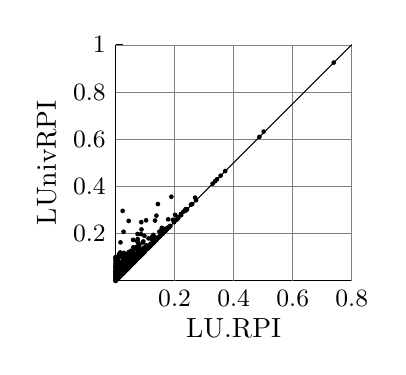
\begin{tikzpicture}

\draw (0,0) -- (3,0);
\node at (1.5,-0.6) {LU.RPI};
\node [anchor=north] at (0.75,0) {\small 0.2};
\draw (0.75,0) -- (0.75,0.1);
\draw [style=help lines] (0.75,0) -- (0.75,3);
\node [anchor=north] at (1.5,0) {\small 0.4};
\draw (1.5,0) -- (1.5,0.1);
\draw [style=help lines] (1.5,0) -- (1.5,3);
\node [anchor=north] at (2.25,0) {\small 0.6};
\draw (2.25,0) -- (2.25,0.1);
\draw [style=help lines] (2.25,0) -- (2.25,3);
\node [anchor=north] at (3,0) {\small 0.8};
\draw (3,0) -- (3,0.1);
\draw [style=help lines] (3,0) -- (3,3);
\draw (0,0) -- (0,3);
\node [rotate=90] at (-2.5em,1.5) {LUnivRPI};
\node [anchor=east] at (0,0.599) {\small 0.2};
\draw (0,0.599) -- (0.1,0.599);
\draw [style=help lines] (0,0.599) -- (3,0.599);
\node [anchor=east] at (0,1.198) {\small 0.4};
\draw (0,1.198) -- (0.1,1.198);
\draw [style=help lines] (0,1.198) -- (3,1.198);
\node [anchor=east] at (0,1.797) {\small 0.6};
\draw (0,1.797) -- (0.1,1.797);
\draw [style=help lines] (0,1.797) -- (3,1.797);
\node [anchor=east] at (0,2.396) {\small 0.8};
\draw (0,2.396) -- (0.1,2.396);
\draw [style=help lines] (0,2.396) -- (3,2.396);
\node [anchor=east] at (0,2.995) {\small 1};
\draw (0,2.995) -- (0.1,2.995);
\draw [style=help lines] (0,2.995) -- (3,2.995);
\foreach \pos in {
	(0.000000, 0.000000),
	(0.004367, 0.004367),
	(0.000000, 0.010490),
	(0.009009, 0.009009),
	(0.005300, 0.015901),
	(0.013333, 0.013333),
	(0.000000, 0.020408),
	(0.007344, 0.022032),
	(0.013363, 0.020045),
	(0.000000, 0.026882),
	(0.019405, 0.019405),
	(0.013550, 0.026197),
	(0.019874, 0.025552),
	(0.010545, 0.031634),
	(0.018545, 0.031636),
	(0.025974, 0.025974),
	(0.000000, 0.039063),
	(0.025373, 0.032836),
	(0.018394, 0.037707),
	(0.031185, 0.031185),
	(0.004545, 0.045455),
	(0.025199, 0.039059),
	(0.014706, 0.044118),
	(0.031370, 0.037975),
	(0.022222, 0.044444),
	(0.029126, 0.043689),
	(0.037514, 0.037514),
	(0.013756, 0.051586),
	(0.024965, 0.049931),
	(0.035319, 0.043629),
	(0.000000, 0.057143),
	(0.018544, 0.056083),
	(0.032504, 0.049358),
	(0.041806, 0.041806),
	(0.038687, 0.049238),
	(0.031774, 0.055605),
	(0.016529, 0.061983),
	(0.023281, 0.060209),
	(0.045596, 0.046526),
	(0.006696, 0.066964),
	(0.039003, 0.055255),
	(0.000000, 0.068571),
	(0.044633, 0.052604),
	(0.012821, 0.068376),
	(0.032098, 0.061848),
	(0.050346, 0.050346),
	(0.024150, 0.067084),
	(0.038633, 0.062407),
	(0.045249, 0.058824),
	(0.032609, 0.068182),
	(0.051980, 0.056436),
	(0.007692, 0.076923),
	(0.017266, 0.075540),
	(0.026026, 0.074074),
	(0.044056, 0.065035),
	(0.038710, 0.070968),
	(0.050669, 0.063336),
	(0.032518, 0.074326),
	(0.000000, 0.081571),
	(0.057884, 0.057884),
	(0.048237, 0.069573),
	(0.056680, 0.064777),
	(0.038541, 0.077081),
	(0.062169, 0.062169),
	(0.044843, 0.076233),
	(0.055670, 0.071134),
	(0.051040, 0.076560),
	(0.062092, 0.068627),
	(0.039669, 0.084298),
	(0.012371, 0.092784),
	(0.031250, 0.088542),
	(0.046997, 0.082245),
	(0.000000, 0.094737),
	(0.021583, 0.093525),
	(0.057252, 0.077290),
	(0.068311, 0.068311),
	(0.064439, 0.074463),
	(0.053834, 0.083197),
	(0.044355, 0.088710),
	(0.037480, 0.092140),
	(0.007732, 0.100515),
	(0.000000, 0.102273),
	(0.063299, 0.080563),
	(0.070661, 0.074380),
	(0.032653, 0.097959),
	(0.019531, 0.101562),
	(0.052678, 0.089552),
	(0.041763, 0.097448),
	(0.013216, 0.105727),
	(0.069543, 0.081133),
	(0.060287, 0.088995),
	(0.076194, 0.076730),
	(0.028754, 0.105431),
	(0.000000, 0.110656),
	(0.048387, 0.099620),
	(0.068465, 0.087137),
	(0.056354, 0.096133),
	(0.075997, 0.083597),
	(0.063315, 0.094398),
	(0.020814, 0.112217),
	(0.043307, 0.106299),
	(0.005894, 0.114931),
	(0.031250, 0.111111),
	(0.082120, 0.082120),
	(0.053088, 0.103467),
	(0.074447, 0.090543),
	(0.062016, 0.100775),
	(0.040036, 0.112100),
	(0.025424, 0.116949),
	(0.080873, 0.088575),
	(0.000000, 0.120000),
	(0.069740, 0.098109),
	(0.051241, 0.109315),
	(0.086692, 0.086692),
	(0.076923, 0.096154),
	(0.012903, 0.122581),
	(0.031447, 0.119497),
	(0.061141, 0.108016),
	(0.083228, 0.094578),
	(0.041152, 0.119342),
	(0.068666, 0.106551),
	(0.056897, 0.113793),
	(0.074353, 0.103448),
	(0.050562, 0.117978),
	(0.002568, 0.128425),
	(0.091082, 0.091082),
	(0.081818, 0.102273),
	(0.089029, 0.097122),
	(0.064000, 0.116000),
	(0.070423, 0.112676),
	(0.076867, 0.109810),
	(0.027815, 0.131126),
	(0.016667, 0.133333),
	(0.095588, 0.095588),
	(0.056133, 0.124740),
	(0.082873, 0.108919),
	(0.088710, 0.104839),
	(0.037736, 0.132075),
	(0.047771, 0.128981),
	(0.069638, 0.119777),
	(0.077381, 0.116071),
	(0.095112, 0.103038),
	(0.101449, 0.097826),
	(0.087800, 0.112463),
	(0.068581, 0.125733),
	(0.055147, 0.132353),
	(0.083937, 0.117150),
	(0.076110, 0.122622),
	(0.000000, 0.145374),
	(0.100313, 0.106583),
	(0.095785, 0.111111),
	(0.024974, 0.146722),
	(0.088995, 0.120574),
	(0.106322, 0.106322),
	(0.078750, 0.128250),
	(0.102094, 0.112565),
	(0.072331, 0.134328),
	(0.096642, 0.118421),
	(0.108247, 0.112113),
	(0.089313, 0.128244),
	(0.061100, 0.144603),
	(0.069124, 0.141014),
	(0.102981, 0.119241),
	(0.095553, 0.126202),
	(0.057508, 0.150160),
	(0.083333, 0.137821),
	(0.114044, 0.114044),
	(0.109091, 0.119580),
	(0.078303, 0.141925),
	(0.102439, 0.125854),
	(0.000000, 0.164234),
	(0.099321, 0.132428),
	(0.091537, 0.138169),
	(0.115963, 0.120258),
	(0.111603, 0.125775),
	(0.107034, 0.129969),
	(0.048649, 0.162162),
	(0.035176, 0.165829),
	(0.064815, 0.157407),
	(0.072041, 0.154374),
	(0.098131, 0.140187),
	(0.086411, 0.148449),
	(0.121919, 0.121919),
	(0.106017, 0.137536),
	(0.058099, 0.163732),
	(0.114645, 0.131379),
	(0.092923, 0.150154),
	(0.123322, 0.128356),
	(0.101266, 0.146835),
	(0.079937, 0.159875),
	(0.070968, 0.164516),
	(0.108216, 0.144289),
	(0.117455, 0.137031),
	(0.000000, 0.180516),
	(0.064549, 0.169057),
	(0.123364, 0.134579),
	(0.129405, 0.129405),
	(0.089457, 0.159744),
	(0.115279, 0.142726),
	(0.058172, 0.174515),
	(0.076807, 0.167169),
	(0.101485, 0.153465),
	(0.082797, 0.165593),
	(0.112957, 0.149502),
	(0.123203, 0.141684),
	(0.131300, 0.135279),
	(0.103752, 0.160522),
	(0.109464, 0.157355),
	(0.036036, 0.189189),
	(0.064994, 0.181300),
	(0.115243, 0.155701),
	(0.130321, 0.143354),
	(0.089503, 0.172376),
	(0.137931, 0.137931),
	(0.123377, 0.152597),
	(0.105882, 0.167647),
	(0.130977, 0.149688),
	(0.098811, 0.172919),
	(0.136153, 0.145436),
	(0.073171, 0.185976),
	(0.120000, 0.160000),
	(0.000000, 0.200000),
	(0.087097, 0.180645),
	(0.114343, 0.165496),
	(0.142857, 0.142857),
	(0.050251, 0.195980),
	(0.104690, 0.174204),
	(0.129114, 0.159494),
	(0.080153, 0.188931),
	(0.141579, 0.148902),
	(0.121896, 0.165914),
	(0.072581, 0.193548),
	(0.091037, 0.186309),
	(0.147541, 0.147541),
	(0.104558, 0.180965),
	(0.140461, 0.157233),
	(0.079439, 0.196262),
	(0.146341, 0.154044),
	(0.099338, 0.188742),
	(0.131918, 0.168309),
	(0.126923, 0.173077),
	(0.152098, 0.152098),
	(0.105606, 0.187744),
	(0.143609, 0.163715),
	(0.151007, 0.158557),
	(0.138462, 0.171041),
	(0.076043, 0.208504),
	(0.157022, 0.157022),
	(0.000000, 0.222222),
	(0.082695, 0.206738),
	(0.114607, 0.191011),
	(0.130035, 0.182969),
	(0.152968, 0.164384),
	(0.058496, 0.217270),
	(0.147368, 0.171053),
	(0.101983, 0.203966),
	(0.159151, 0.164456),
	(0.037696, 0.226178),
	(0.126667, 0.191667),
	(0.140244, 0.182927),
	(0.153696, 0.173152),
	(0.146341, 0.180775),
	(0.110400, 0.206400),
	(0.165517, 0.165517),
	(0.162562, 0.171429),
	(0.157895, 0.179825),
	(0.081720, 0.225806),
	(0.169811, 0.169811),
	(0.138500, 0.197857),
	(0.130796, 0.203460),
	(0.165000, 0.177500),
	(0.073952, 0.231717),
	(0.091640, 0.226688),
	(0.160305, 0.186478),
	(0.036855, 0.243243),
	(0.117383, 0.217447),
	(0.174832, 0.174832),
	(0.147241, 0.198888),
	(0.170616, 0.180095),
	(0.141768, 0.205793),
	(0.166768, 0.186927),
	(0.111570, 0.226240),
	(0.000000, 0.252632),
	(0.137405, 0.213740),
	(0.176471, 0.183007),
	(0.156904, 0.202406),
	(0.106401, 0.233564),
	(0.174194, 0.188710),
	(0.148897, 0.209559),
	(0.018979, 0.257569),
	(0.126246, 0.225914),
	(0.184265, 0.185645),
	(0.172748, 0.198404),
	(0.143089, 0.221138),
	(0.179919, 0.194070),
	(0.087549, 0.250973),
	(0.159218, 0.213687),
	(0.186090, 0.191729),
	(0.172708, 0.204691),
	(0.155620, 0.220461),
	(0.192913, 0.192913),
	(0.173021, 0.214076),
	(0.166667, 0.219807),
	(0.196144, 0.198659),
	(0.188247, 0.206175),
	(0.161448, 0.228963),
	(0.000000, 0.281250),
	(0.179543, 0.218716),
	(0.174515, 0.224377),
	(0.196721, 0.206557),
	(0.190733, 0.213362),
	(0.203103, 0.203103),
	(0.171912, 0.230255),
	(0.164122, 0.236641),
	(0.186441, 0.220339),
	(0.199434, 0.212164),
	(0.000000, 0.291262),
	(0.032258, 0.290323),
	(0.102857, 0.274286),
	(0.147082, 0.254475),
	(0.207242, 0.209385),
	(0.193746, 0.222298),
	(0.187500, 0.228659),
	(0.155405, 0.252252),
	(0.175127, 0.239502),
	(0.000000, 0.300000),
	(0.202222, 0.222222),
	(0.212085, 0.213270),
	(0.161815, 0.256849),
	(0.183414, 0.245157),
	(0.144695, 0.270096),
	(0.100000, 0.290000),
	(0.214651, 0.219761),
	(0.209607, 0.229258),
	(0.186158, 0.250597),
	(0.152406, 0.272727),
	(0.201705, 0.238636),
	(0.058906, 0.307153),
	(0.221352, 0.222331),
	(0.218373, 0.228163),
	(0.115481, 0.298745),
	(0.226619, 0.226619),
	(0.218613, 0.234416),
	(0.139535, 0.290698),
	(0.215548, 0.240283),
	(0.132813, 0.296875),
	(0.226929, 0.236006),
	(0.231984, 0.231984),
	(0.187879, 0.269697),
	(0.176471, 0.277311),
	(0.216190, 0.248766),
	(0.199367, 0.265823),
	(0.140318, 0.303087),
	(0.109261, 0.316857),
	(0.064516, 0.329032),
	(0.237251, 0.237251),
	(0.158654, 0.295673),
	(0.227538, 0.248541),
	(0.043668, 0.336245),
	(0.191411, 0.280982),
	(0.235075, 0.246269),
	(0.227891, 0.258503),
	(0.118705, 0.323741),
	(0.243958, 0.243958),
	(0.240810, 0.250938),
	(0.248040, 0.250178),
	(0.237617, 0.262165),
	(0.201622, 0.292005),
	(0.230769, 0.270243),
	(0.131542, 0.330976),
	(0.248189, 0.257278),
	(0.254325, 0.254325),
	(0.236659, 0.271462),
	(0.210291, 0.293065),
	(0.058824, 0.358289),
	(0.253898, 0.260579),
	(0.169231, 0.323077),
	(0.221591, 0.289773),
	(0.246938, 0.271926),
	(0.205319, 0.306520),
	(0.105263, 0.354067),
	(0.254672, 0.272290),
	(0.250319, 0.278416),
	(0.155709, 0.342561),
	(0.261307, 0.271357),
	(0.210913, 0.317943),
	(0.258845, 0.281588),
	(0.268408, 0.274660),
	(0.247633, 0.296431),
	(0.164948, 0.350515),
	(0.269118, 0.282353),
	(0.277142, 0.280612),
	(0.239244, 0.317943),
	(0.264770, 0.298770),
	(0.168717, 0.363796),
	(0.212286, 0.340591),
	(0.283951, 0.283951),
	(0.279141, 0.291411),
	(0.249370, 0.317380),
	(0.287571, 0.288790),
	(0.265165, 0.311958),
	(0.210402, 0.352246),
	(0.283113, 0.298013),
	(0.288703, 0.294979),
	(0.275902, 0.310827),
	(0.240711, 0.345719),
	(0.215617, 0.362023),
	(0.284424, 0.311512),
	(0.298747, 0.298747),
	(0.282723, 0.321990),
	(0.303598, 0.303598),
	(0.198748, 0.381847),
	(0.219101, 0.375000),
	(0.308964, 0.308964),
	(0.299220, 0.320808),
	(0.311100, 0.315789),
	(0.304147, 0.325872),
	(0.299177, 0.332113),
	(0.313433, 0.326866),
	(0.320900, 0.320900),
	(0.304718, 0.344037),
	(0.326425, 0.326425),
	(0.286082, 0.363402),
	(0.329558, 0.331823),
	(0.315517, 0.346552),
	(0.245758, 0.405500),
	(0.334153, 0.336481),
	(0.259375, 0.403125),
	(0.339950, 0.339950),
	(0.226212, 0.425494),
	(0.336909, 0.346372),
	(0.318277, 0.371849),
	(0.346776, 0.347547),
	(0.062593, 0.487332),
	(0.339768, 0.355212),
	(0.312461, 0.383260),
	(0.352941, 0.352941),
	(0.312599, 0.396989),
	(0.354227, 0.362974),
	(0.303797, 0.406872),
	(0.269164, 0.431185),
	(0.322008, 0.393822),
	(0.337748, 0.384106),
	(0.362745, 0.362745),
	(0.368852, 0.368852),
	(0.373610, 0.373610),
	(0.355536, 0.391869),
	(0.352518, 0.402878),
	(0.373989, 0.387863),
	(0.366838, 0.394823),
	(0.302178, 0.454628),
	(0.380041, 0.397149),
	(0.356890, 0.418728),
	(0.288312, 0.479221),
	(0.381215, 0.414365),
	(0.223118, 0.518817),
	(0.401936, 0.401936),
	(0.397554, 0.406728),
	(0.277014, 0.498035),
	(0.402672, 0.412214),
	(0.408727, 0.408727),
	(0.277710, 0.507917),
	(0.406977, 0.423256),
	(0.417994, 0.419088),
	(0.390733, 0.448967),
	(0.414600, 0.429483),
	(0.346939, 0.486395),
	(0.280665, 0.530146),
	(0.426829, 0.426829),
	(0.412541, 0.442244),
	(0.419624, 0.438413),
	(0.352941, 0.499160),
	(0.438213, 0.439599),
	(0.444500, 0.444500),
	(0.102273, 0.622159),
	(0.439739, 0.459283),
	(0.457012, 0.462020),
	(0.447280, 0.471457),
	(0.279534, 0.594010),
	(0.472072, 0.472072),
	(0.323544, 0.592405),
	(0.478431, 0.478431),
	(0.366848, 0.570652),
	(0.418803, 0.538462),
	(0.485581, 0.485581),
	(0.456221, 0.530876),
	(0.495146, 0.509709),
	(0.508130, 0.508130),
	(0.462236, 0.552870),
	(0.515304, 0.515304),
	(0.329557, 0.651724),
	(0.486435, 0.556467),
	(0.500000, 0.551282),
	(0.530574, 0.533396),
	(0.479458, 0.581758),
	(0.534354, 0.544858),
	(0.541339, 0.549213),
	(0.167102, 0.759791),
	(0.549662, 0.552555),
	(0.566875, 0.567790),
	(0.566994, 0.574067),
	(0.326656, 0.744222),
	(0.581419, 0.596404),
	(0.586279, 0.591913),
	(0.557185, 0.624633),
	(0.592893, 0.592893),
	(0.598803, 0.600378),
	(0.583914, 0.617694),
	(0.605854, 0.605854),
	(0.387597, 0.767442),
	(0.627142, 0.627142),
	(0.590070, 0.662635),
	(0.089888, 0.887640),
	(0.628999, 0.633153),
	(0.588167, 0.671694),
	(0.637417, 0.637417),
	(0.501528, 0.764732),
	(0.640533, 0.662722),
	(0.655066, 0.656275),
	(0.664245, 0.671352),
	(0.675813, 0.675813),
	(0.681072, 0.682819),
	(0.519183, 0.826939),
	(0.691057, 0.691057),
	(0.696561, 0.696870),
	(0.669130, 0.780000),
	(0.743390, 0.743390),
	(0.743363, 0.750603),
	(0.728400, 0.774335),
	(0.772600, 0.772600),
	(0.538050, 0.973996),
	(0.790795, 0.790795),
	(0.756032, 0.836461),
	(0.797386, 0.799020),
	(0.790571, 0.808437),
	(0.833239, 0.833239),
	(0.829088, 0.847749),
	(0.861519, 0.877792),
	(0.889159, 0.889507),
	(0.888000, 0.896000),
	(0.887715, 0.907530),
	(0.900283, 0.900283),
	(0.708972, 1.066740),
	(0.909224, 0.909224),
	(0.958415, 0.967221),
	(0.973150, 0.973150),
	(1.023024, 1.023024),
	(1.010802, 1.055671),
	(1.232750, 1.232750),
	(1.264940, 1.264940),
	(1.289613, 1.289613),
	(1.334389, 1.334389),
	(1.393080, 1.393080),
	(1.827128, 1.827128),
	(1.881198, 1.894112),
	(2.770800, 2.770800),
} \fill \pos circle(0.03);
\draw (0,0) -- (3, 3);
\end{tikzpicture}

  } \
  \subfloat[Compression ratio difference]{
    \centering
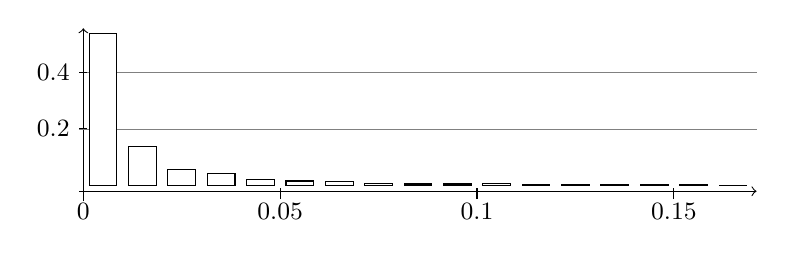
\begin{tikzpicture}
\draw[->] (-0.25,-0.2) -- (-0.25,2);
\draw [style=help lines] (-0.3,0.720894419908818) -- (8.3,0.720894419908818);
\node [anchor=east,fill=white] at (-0.3,0.720894419908818) {\small 0.2};
\draw (-0.3,0.720894419908818) -- (-0.2,0.720894419908818);
\draw [style=help lines] (-0.3,1.44178883981764) -- (8.3,1.44178883981764);
\node [anchor=east,fill=white] at (-0.3,1.44178883981764) {\small 0.4};
\draw (-0.3,1.44178883981764) -- (-0.2,1.44178883981764);
\draw[->] (-0.3,-0.07) -- (8.3,-0.07);
\node [anchor=north] at (-0.25, -0.1) {\small 0};
\draw (-0.25,-0.17) -- (-0.25,-0.03);
\node [anchor=north] at (2.25, -0.1) {\small 0.05};
\draw (2.25,-0.17) -- (2.25,-0.03);
\node [anchor=north] at (4.75, -0.1) {\small 0.1};
\draw (4.75,-0.17) -- (4.75,-0.03);
\node [anchor=north] at (7.25, -0.1) {\small 0.15};
\draw (7.25,-0.17) -- (7.25,-0.03);

\draw[fill=white] plot[ybar] coordinates {
	(6.000000, 0.011416)
	(6.500000, 0.009989)
	(7.500000, 0.011416)
	(3.000000, 0.047803)
	(5.500000, 0.017837)
	(5.000000, 0.024972)
	(8.000000, 0.002854)
	(1.500000, 0.151257)
	(4.500000, 0.021404)
	(3.500000, 0.028539)
	(0.500000, 0.492298)
	(0.000000, 1.927811)
	(4.000000, 0.022118)
	(2.500000, 0.059932)
	(1.000000, 0.209048)
	(2.000000, 0.077769)
	(7.000000, 0.010702)
};

\end{tikzpicture}
  } \
  \subfloat[Duration difference]{
    \centering
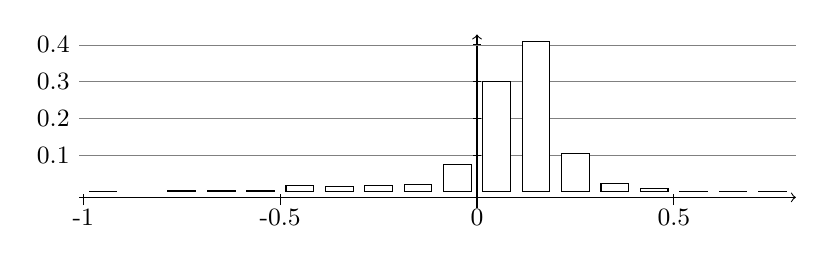
\begin{tikzpicture}
\draw[->] (-0.25,-0.2) -- (-0.25,2);
\draw [style=help lines] (-5.3,0.466521185853302) -- (3.8,0.466521185853302);
\node [anchor=east,fill=white] at (-5.3,0.466521185853302) {\small 0.1};
\draw (-0.3,0.466521185853302) -- (-0.2,0.466521185853302);
\draw [style=help lines] (-5.3,0.933042371706605) -- (3.8,0.933042371706605);
\node [anchor=east,fill=white] at (-5.3,0.933042371706605) {\small 0.2};
\draw (-0.3,0.933042371706605) -- (-0.2,0.933042371706605);
\draw [style=help lines] (-5.3,1.39956355755991) -- (3.8,1.39956355755991);
\node [anchor=east,fill=white] at (-5.3,1.39956355755991) {\small 0.3};
\draw (-0.3,1.39956355755991) -- (-0.2,1.39956355755991);
\draw [style=help lines] (-5.3,1.86608474341321) -- (3.8,1.86608474341321);
\node [anchor=east,fill=white] at (-5.3,1.86608474341321) {\small 0.4};
\draw (-0.3,1.86608474341321) -- (-0.2,1.86608474341321);
\draw[->] (-5.3,-0.07) -- (3.8,-0.07);
\node [anchor=north] at (-5.25, -0.1) {\small -1};
\draw (-5.25,-0.17) -- (-5.25,-0.03);
\node [anchor=north] at (-2.75, -0.1) {\small -0.5};
\draw (-2.75,-0.17) -- (-2.75,-0.03);
\node [anchor=north] at (-0.25, -0.1) {\small 0};
\draw (-0.25,-0.17) -- (-0.25,-0.03);
\node [anchor=north] at (2.25, -0.1) {\small 0.5};
\draw (2.25,-0.17) -- (2.25,-0.03);

\draw[fill=white] plot[ybar] coordinates {
	(1.000000, 0.485172)
	(-4.000000, 0.015710)
	(3.500000, 0.000924)
	(1.500000, 0.100731)
	(0.000000, 1.404689)
	(2.000000, 0.038814)
	(-3.500000, 0.017559)
	(0.500000, 1.906496)
	(-0.500000, 0.352096)
	(-3.000000, 0.019407)
	(3.000000, 0.006469)
	(-2.000000, 0.065614)
	(-1.000000, 0.095186)
	(2.500000, 0.004621)
	(-1.500000, 0.081324)
	(-5.000000, 0.000924)
	(-2.500000, 0.076703)
};

\end{tikzpicture}
  }
  \caption{Comparison between LU.RPI and LUnivRPI}
  \label{fig:LUnivRPI}
\end{figure}




\section{Conclusions and Future Work}

{\LowerUnivalents}, the algorithm presented here, has been shown in the previous section to compress
more than {\LowerUnits}. This is so because, as demonstrated in Proposition \ref{prop:compression}, the
set of subproofs it lowers is always a superset of the set of subproofs lowered by {\LowerUnits}. It might
be possible to lower even more subproofs by finding a characterization of (efficiently) lowerable subproofs
broader than that of univalent subproofs considered here. This direction for future work promises to be challenging, though, as evidenced by the non-triviality of the optimizations discussed in Section \ref{sec:LUniv} for obtaining a linear-time implementation of {\LowerUnivalents}.

As discussed in Section \ref{sec:LUnivRPI}, the proposed algorithm can be embedded in the deletion traversal of other algorithms.  As
an example, it has been shown that the combination of {\LowerUnivalents} with {\RPI}, compared to
the sequential composition of {\LowerUnits} after {\RPI}, results in a better compression ratio with
only a small processing time overhead (Figure \ref{fig:LUnivRPI}). Other compression algorithms that also have a subproof
deletion or reconstruction phase (e.g. \ReduceReconstruct) could probably benefit from being
combined with {\LowerUnivalents} as well.



\paragraph{Acknowledgments:}

The authors would like to thank Pascal Fontaine for providing {\veriT}'s proofs for the experiments,
for co-organizing our joint workshops on proof
compression\footnote{\url{http://www.logic.at/people/bruno/MediaWiki/index.php/Amadeus_Vienna-Nancy_Joint_Project_on_Proof_Compression}},
and for several interesting and useful discussions on this topic.


\bibliographystyle{splncs}
\bibliography{../biblio}


\end{document}

% vim: tw=100
